%% ABS challenges: wins left on the table. Every number is a macro from generated/numbers.tex
%% (paper/make_numbers.py reads results/); build with make -C paper. `make submission` writes main-flat.tex with all
%% \input{}s expanded, as AoAS asks for one .tex file.
\documentclass[aoas]{imsart}

\RequirePackage{amsthm,amsmath,amsfonts,amssymb}
\RequirePackage[authoryear]{natbib}
\RequirePackage{xurl}
\RequirePackage[colorlinks,citecolor=blue,urlcolor=blue,pdftitle={ABS challenges: wins left on the table},
  pdfauthor={Jan Janou\v{s}ek and Michal Pe\v{s}ta}]{hyperref}
\RequirePackage{graphicx,booktabs}

\startlocaldefs
\theoremstyle{plain}
\newtheorem{theorem}{Theorem}
\newtheorem{proposition}[theorem]{Proposition}
\newtheorem{lemma}[theorem]{Lemma}
\theoremstyle{definition}
\newtheorem{assumption}{Assumption}
\newtheorem{remark}{Remark}
\newcommand{\E}{\mathbb{E}}
\newcommand{\Prob}{\mathbb{P}}
\setcounter{secnumdepth}{3}
% generated by paper/make_numbers.py from results/ -- do not edit
\newcommand{\AAASrBatter}{3.22}
\newcommand{\AAASrCatcher}{2.09}
\newcommand{\AAASrPctHi}{15}
\newcommand{\AAASrPctLo}{12}
\newcommand{\BGTopChExcess}{25}
\newcommand{\BGTopValueExcess}{0.02}
\newcommand{\BGValueExpected}{3.32}
\newcommand{\BGValueObserved}{3.34}
\newcommand{\BICMain}{55{,}329}
\newcommand{\BICRE}{54{,}049}
\newcommand{\BICRELapse}{54{,}035}
\newcommand{\BICSmoothMinusDet}{58}
\newcommand{\BinaryLost}{0.68}
\newcommand{\BinaryLostCI}{[0.57, 0.80]}
\newcommand{\BinaryMinusRB}{\ensuremath{-}0.008}
\newcommand{\BinaryMinusRBCI}{[\ensuremath{-}0.025, 0.009]}
\newcommand{\BinaryMinusRBSimAbs}{0.00}
\newcommand{\BlockBootB}{100}
\newcommand{\BlockBootCI}{[0.54, 0.78]}
\newcommand{\BreakEvenLLBatter}{73}
\newcommand{\BreakEvenLLCatcher}{133}
\newcommand{\BreakEvenPct}{20}
\newcommand{\CIEndSE}{0.008}
\newcommand{\CPLapseB}{50}
\newcommand{\CPLapseBasic}{17}
\newcommand{\CPLapseBias}{0.162}
\newcommand{\CPLapseBiasK}{0.212}
\newcommand{\CPLapseBiasSE}{0.010}
\newcommand{\CPLapseBootSD}{0.064}
\newcommand{\CPLapseGap}{0.57}
\newcommand{\CPLapseGapK}{0.52}
\newcommand{\CPLapseKBasic}{7}
\newcommand{\CPLapseKNormal}{10}
\newcommand{\CPLapseKPct}{10}
\newcommand{\CPLapseKPctCI}{[2, 27]}
\newcommand{\CPLapseLearn}{0.05}
\newcommand{\CPLapseMissHigh}{21}
\newcommand{\CPLapseMissLow}{0}
\newcommand{\CPLapseNormal}{23}
\newcommand{\CPLapsePct}{30}
\newcommand{\CPLapsePctCI}{[15, 49]}
\newcommand{\CPLapsePointSD}{0.055}
\newcommand{\CPLapseS}{30}
\newcommand{\CPMainB}{50}
\newcommand{\CPMainBasic}{90}
\newcommand{\CPMainBias}{\ensuremath{-}0.037}
\newcommand{\CPMainBiasK}{\ensuremath{-}0.032}
\newcommand{\CPMainBiasSE}{0.008}
\newcommand{\CPMainBootSD}{0.064}
\newcommand{\CPMainGap}{0.70}
\newcommand{\CPMainGapK}{0.69}
\newcommand{\CPMainKBasic}{88}
\newcommand{\CPMainKNormal}{90}
\newcommand{\CPMainKPct}{92}
\newcommand{\CPMainKPctCI}{[81, 98]}
\newcommand{\CPMainLearn}{0.01}
\newcommand{\CPMainMissHigh}{0}
\newcommand{\CPMainMissLow}{4}
\newcommand{\CPMainNormal}{90}
\newcommand{\CPMainPct}{92}
\newcommand{\CPMainPctCI}{[81, 98]}
\newcommand{\CPMainPointSD}{0.055}
\newcommand{\CPMainS}{50}
\newcommand{\CPMisB}{20}
\newcommand{\CPMisBasic}{50}
\newcommand{\CPMisBias}{\ensuremath{-}0.072}
\newcommand{\CPMisBiasK}{\ensuremath{-}0.001}
\newcommand{\CPMisBiasSE}{0.012}
\newcommand{\CPMisBootSD}{0.066}
\newcommand{\CPMisGap}{0.78}
\newcommand{\CPMisGapK}{0.71}
\newcommand{\CPMisKBasic}{92}
\newcommand{\CPMisKNormal}{100}
\newcommand{\CPMisKPct}{92}
\newcommand{\CPMisKPctCI}{[62, 100]}
\newcommand{\CPMisLearn}{0.07}
\newcommand{\CPMisMissHigh}{0}
\newcommand{\CPMisMissLow}{0}
\newcommand{\CPMisNormal}{92}
\newcommand{\CPMisPct}{100}
\newcommand{\CPMisPctCI}{[74, 100]}
\newcommand{\CPMisPointSD}{0.040}
\newcommand{\CPMisS}{12}
\newcommand{\CPPrimB}{30}
\newcommand{\CPPrimBasic}{50}
\newcommand{\CPPrimBias}{\ensuremath{-}0.069}
\newcommand{\CPPrimBiasK}{0.009}
\newcommand{\CPPrimBiasSE}{0.011}
\newcommand{\CPPrimBootSD}{0.063}
\newcommand{\CPPrimGap}{0.65}
\newcommand{\CPPrimGapK}{0.57}
\newcommand{\CPPrimKBasic}{80}
\newcommand{\CPPrimKNormal}{100}
\newcommand{\CPPrimKPct}{80}
\newcommand{\CPPrimKPctCI}{[61, 92]}
\newcommand{\CPPrimLearn}{0.08}
\newcommand{\CPPrimMissHigh}{0}
\newcommand{\CPPrimMissLow}{4}
\newcommand{\CPPrimNormal}{77}
\newcommand{\CPPrimPct}{87}
\newcommand{\CPPrimPctCI}{[69, 96]}
\newcommand{\CPPrimPointSD}{0.061}
\newcommand{\CPPrimS}{30}
\newcommand{\CPREB}{50}
\newcommand{\CPREBasic}{43}
\newcommand{\CPREBias}{0.095}
\newcommand{\CPREBiasK}{0.160}
\newcommand{\CPREBiasSE}{0.009}
\newcommand{\CPREBootSD}{0.064}
\newcommand{\CPREGap}{0.65}
\newcommand{\CPREGapK}{0.58}
\newcommand{\CPREKBasic}{23}
\newcommand{\CPREKNormal}{27}
\newcommand{\CPREKPct}{37}
\newcommand{\CPREKPctCI}{[20, 56]}
\newcommand{\CPRELearn}{0.07}
\newcommand{\CPREMissHigh}{4}
\newcommand{\CPREMissLow}{0}
\newcommand{\CPRENormal}{70}
\newcommand{\CPREPct}{87}
\newcommand{\CPREPctCI}{[69, 96]}
\newcommand{\CPREPointSD}{0.052}
\newcommand{\CPRES}{30}
\newcommand{\CausalBootN}{2{,}000}
\newcommand{\CausalK}{1000}
\newcommand{\CausalMinusPath}{0.000}
\newcommand{\CausalMinusPathCI}{[\ensuremath{-}0.002, 0.002]}
\newcommand{\CausalR}{10}
\newcommand{\CausalSkipShare}{47}
\newcommand{\ClairGap}{0.81}
\newcommand{\CoB}{400}
\newcommand{\CoLost}{0.55}
\newcommand{\CoLostCI}{[0.36, 0.72]}
\newcommand{\CoLostRemoved}{0.91}
\newcommand{\CoShareRule}{95.4}
\newcommand{\ContamPct}{0.05}
\newcommand{\CovB}{20}
\newcommand{\CovBMis}{10}
\newcommand{\CovBootSD}{0.071}
\newcommand{\CovGap}{0.72}
\newcommand{\CovLapseBias}{0.15}
\newcommand{\CovLapseGap}{0.60}
\newcommand{\CovLapseNormal}{45}
\newcommand{\CovLapseRate}{32}
\newcommand{\CovLapseS}{22}
\newcommand{\CovMainBasic}{80}
\newcommand{\CovMainBias}{\ensuremath{-}0.055}
\newcommand{\CovMainBiasAbs}{0.06}
\newcommand{\CovMainMissHigh}{0}
\newcommand{\CovMainMissLow}{10}
\newcommand{\CovMainNormal}{90}
\newcommand{\CovMainRate}{80}
\newcommand{\CovMainRateCI}{[66.3, 90.0]}
\newcommand{\CovPointSD}{0.061}
\newcommand{\CovR}{2}
\newcommand{\CovREBias}{0.06}
\newcommand{\CovREGap}{0.68}
\newcommand{\CovRENormal}{85}
\newcommand{\CovRERate}{73}
\newcommand{\CovRES}{26}
\newcommand{\CovS}{50}
\newcommand{\CovSMis}{30}
\newcommand{\CovTruthStreams}{16}
\newcommand{\CrossFive}{27}
\newcommand{\CrossThree}{10}
\newcommand{\CrossTwo}{4}
\newcommand{\CurseBias}{0.07}
\newcommand{\CurseBiasSD}{0.01}
\newcommand{\CurseLostCross}{0.65}
\newcommand{\CurseLostSame}{0.72}
\newcommand{\DLLEdge}{193}
\newcommand{\DLLMain}{355}
\newcommand{\DLLRE}{1{,}032}
\newcommand{\DLLREvsMain}{679}
\newcommand{\DLLRejHi}{854}
\newcommand{\DLLRejLo}{107}
\newcommand{\DLLRejMainHi}{893}
\newcommand{\DLLRejMainLo}{126}
\newcommand{\DPConcEntPct}{0.6}
\newcommand{\DPConcOppPct}{0.1}
\newcommand{\DPRiseEntPct}{20}
\newcommand{\DPRiseOppPct}{9}
\newcommand{\DRSB}{500}
\newcommand{\DRSMatches}{2{,}279}
\newcommand{\DRSODILBW}{29.0}
\newcommand{\DRSODILost}{0.018}
\newcommand{\DRSODILostObs}{0.00}
\newcommand{\DRSODILostObsCI}{[\ensuremath{-}0.13, 0.44]}
\newcommand{\DRSODIMove}{13}
\newcommand{\DRSODIPower}{1.67}
\newcommand{\DRSODIS}{0.81}
\newcommand{\DRSODIShare}{98.5}
\newcommand{\DRSTestLBW}{30.3}
\newcommand{\DRSTestLost}{0.020}
\newcommand{\DRSTestLostObs}{0.13}
\newcommand{\DRSTestLostObsCI}{[\ensuremath{-}0.27, 0.49]}
\newcommand{\DRSTestMove}{18}
\newcommand{\DRSTestPower}{1.66}
\newcommand{\DRSTestS}{0.47}
\newcommand{\DRSTestShare}{99.8}
\newcommand{\DRSTtLBW}{27.8}
\newcommand{\DRSTtLost}{0.001}
\newcommand{\DRSTtLostObs}{0.02}
\newcommand{\DRSTtLostObsCI}{[\ensuremath{-}0.04, 0.09]}
\newcommand{\DRSTtMove}{7}
\newcommand{\DRSTtPower}{1.85}
\newcommand{\DRSTtS}{0.45}
\newcommand{\DRSTtShare}{99.5}
\newcommand{\DecBothGap}{82}
\newcommand{\DecBothGapCI}{[71, 86]}
\newcommand{\DecBothN}{2.39}
\newcommand{\DecBothScaleGap}{79}
\newcommand{\DecBothScaleN}{2.53}
\newcommand{\DecBothScaleShare}{96.5}
\newcommand{\DecBothShare}{96.9}
\newcommand{\DecFitGap}{-6}
\newcommand{\DecFitN}{2.15}
\newcommand{\DecFitShare}{82.4}
\newcommand{\DecIntGap}{53}
\newcommand{\DecIntGapCI}{[38, 61]}
\newcommand{\DecIntN}{2.93}
\newcommand{\DecIntShare}{92.1}
\newcommand{\DecR}{20}
\newcommand{\DecRTune}{10}
\newcommand{\DecStakeBeatsPct}{100}
\newcommand{\DecStakeGap}{81}
\newcommand{\DecStakeGapCI}{[68, 87]}
\newcommand{\DecStakeN}{2.45}
\newcommand{\DecStakeScaleGap}{69}
\newcommand{\DecStakeScaleGapCI}{[59, 80]}
\newcommand{\DecStakeScaleN}{2.33}
\newcommand{\DecStakeScaleShare}{94.9}
\newcommand{\DecStakeShare}{96.9}
\newcommand{\DeltaFirst}{0.017}
\newcommand{\DeltaRatio}{0.53--0.54}
\newcommand{\DeltaSqRTwoAway}{0.9975}
\newcommand{\DeltaSqRTwoHome}{0.9976}
\newcommand{\DetCoordBiasBatter}{0.5}
\newcommand{\DetCoordBiasCatcher}{1.4}
\newcommand{\DetRank}{2}
\newcommand{\DetVersion}{15.0}
\newcommand{\EdgeOrigSlope}{0.84}
\newcommand{\EdgeOrigSlopeCI}{[0.59, 1.09]}
\newcommand{\EdgeOtherSDMax}{0.09}
\newcommand{\EdgeStrikesSD}{0.28}
\newcommand{\ExtraGamesPct}{9}
\newcommand{\FMDeltaCI}{[0.008, 0.009]}
\newcommand{\FMGapClosed}{68}
\newcommand{\FMGapClosedCI}{[61, 75]}
\newcommand{\FarLogGBatter}{0.34}
\newcommand{\FarLogGCatcher}{0.39}
\newcommand{\FarLogGSEBatter}{0.13}
\newcommand{\FarLogGSECatcher}{0.22}
\newcommand{\FarNBatter}{374}
\newcommand{\FarNCatcher}{241}
\newcommand{\FarOneLeftBatter}{\ensuremath{-}0.74}
\newcommand{\FarOneLeftCatcher}{\ensuremath{-}0.92}
\newcommand{\FarOneLeftSEBatter}{0.26}
\newcommand{\FarOneLeftSECatcher}{0.35}
\newcommand{\FarRateBatter}{44}
\newcommand{\FarRateCatcher}{70}
\newcommand{\FarRateOneBatter}{38}
\newcommand{\FarRateOneCatcher}{61}
\newcommand{\FarRateTwoBatter}{46}
\newcommand{\FarRateTwoCatcher}{74}
\newcommand{\FeedBaseSrBatter}{3.11}
\newcommand{\FeedBaseSrCatcher}{1.88}
\newcommand{\FeedSrBatter}{2.90}
\newcommand{\FeedSrCatcher}{1.84}
\newcommand{\FlatBestDelta}{0.008}
\newcommand{\FlatBound}{44.7}
\newcommand{\FlatIdentityGap}{6\times 10^{-17}}
\newcommand{\FlatLocal}{6.5}
\newcommand{\FlatLoss}{6.0}
\newcommand{\FrozenAllDelta}{0.008}
\newcommand{\FrozenDPShare}{99.1}
\newcommand{\FrozenDPShareNoEng}{99.2}
\newcommand{\FrozenDPShareWorldTest}{98.4}
\newcommand{\FrozenDelta}{0.008}
\newcommand{\FrozenGapClosed}{68}
\newcommand{\FrozenLost}{0.48}
\newcommand{\FrozenLostNoEng}{0.48}
\newcommand{\FrozenLostWorldTest}{0.60}
\newcommand{\FrozenR}{20}
\newcommand{\FrozenRuleGapClosed}{64}
\newcommand{\FrozenRuleShareDP}{95.6}
\newcommand{\FrozenRuleShareRetro}{94.7}
\newcommand{\FrozenRuleShareRetroNoEng}{94.7}
\newcommand{\FrozenRuleShareRetroWorldTest}{94.4}
\newcommand{\FrozenShare}{95.7}
\newcommand{\FrozenTestGames}{1{,}146}
\newcommand{\FrozenTrainGames}{1{,}279}
\newcommand{\FullPathObs}{0.69}
\newcommand{\FullPathRule}{0.72}
\newcommand{\FullRB}{0.72}
\newcommand{\FullRBCI}{[0.65, 0.79]}
\newcommand{\FullWin}{0.70}
\newcommand{\FullWinCI}{[0.63, 0.77]}
\newcommand{\Gap}{0.51}
\newcommand{\GapAlgPct}{12}
\newcommand{\GapB}{400}
\newcommand{\GapBFail}{0}
\newcommand{\GapBFailDiff}{0.000}
\newcommand{\GapBFailText}{all fold fits reached the gradient tolerance}
\newcommand{\GapBasic}{[0.35, 0.61]}
\newcommand{\GapBench}{3.85}
\newcommand{\GapBenchCI}{[3.71, 4.06]}
\newcommand{\GapBestDelta}{0.007}
\newcommand{\GapBestShare}{95.5}
\newcommand{\GapBootBias}{0.027}
\newcommand{\GapBootHours}{915}
\newcommand{\GapBootMean}{0.53}
\newcommand{\GapBootMinutes}{137}
\newcommand{\GapBootSD}{0.064}
\newcommand{\GapBootSDAlg}{0.060}
\newcommand{\GapCI}{[0.38, 0.63]}
\newcommand{\GapCalFine}{0.39}
\newcommand{\GapCalFineNauxEight}{0.44}
\newcommand{\GapCardPubGapPct}{60}
\newcommand{\GapCardPubN}{2.54}
\newcommand{\GapCardPubShare}{94.8}
\newcommand{\GapCardRefitGapPct}{56}
\newcommand{\GapCardRefitN}{2.55}
\newcommand{\GapCardRefitShare}{94.2}
\newcommand{\GapDTrainHi}{0.0077}
\newcommand{\GapDTrainLo}{0.0069}
\newcommand{\GapEarlyLateOne}{8.5}
\newcommand{\GapEarlyLateOneCI}{[7.1, 9.8]}
\newcommand{\GapEarlyLateOneDown}{27.3}
\newcommand{\GapEarlyLateOneOcc}{27.5}
\newcommand{\GapEarlyLateOneOccCI}{[26.6, 28.7]}
\newcommand{\GapEarlyLateOneUp}{27.3}
\newcommand{\GapEarlyLateTwo}{12.5}
\newcommand{\GapEarlyLateTwoCI}{[11.5, 13.4]}
\newcommand{\GapEarlyLateTwoDown}{27.7}
\newcommand{\GapEarlyLateTwoOcc}{27.0}
\newcommand{\GapEarlyLateTwoOccCI}{[26.3, 27.7]}
\newcommand{\GapEarlyLateTwoUp}{29.6}
\newcommand{\GapExtS}{8}
\newcommand{\GapFMGapCI}{[53, 72]}
\newcommand{\GapFMGapPct}{63}
\newcommand{\GapFitRuleCI}{[\ensuremath{-}44.7, \ensuremath{-}0.2]}
\newcommand{\GapFitRuleGapPct}{\ensuremath{-}16}
\newcommand{\GapFitRuleN}{2.16}
\newcommand{\GapFitRuleShare}{84.7}
\newcommand{\GapFitRuleWins}{3.26}
\newcommand{\GapFrozenGapCI}{[54, 73]}
\newcommand{\GapFrozenGapPct}{64}
\newcommand{\GapFrozenN}{2.27}
\newcommand{\GapFrozenShare}{95.3}
\newcommand{\GapFrozenWins}{3.67}
\newcommand{\GapGridHi}{2.93}
\newcommand{\GapK}{5}
\newcommand{\GapLamHalf}{0.68}
\newcommand{\GapLamOne}{0.85}
\newcommand{\GapLapse}{0.46}
\newcommand{\GapLeague}{15}
\newcommand{\GapMCSE}{0.013}
\newcommand{\GapMain}{0.63}
\newcommand{\GapMainAlgPct}{9}
\newcommand{\GapMainB}{400}
\newcommand{\GapMainBFail}{22}
\newcommand{\GapMainBFailDiff}{0.002}
\newcommand{\GapMainBFailText}{22 replicates with a fold that did not are kept}
\newcommand{\GapMainBasic}{[0.53, 0.79]}
\newcommand{\GapMainBench}{3.98}
\newcommand{\GapMainBenchCI}{[3.79, 4.11]}
\newcommand{\GapMainBestDelta}{0.008}
\newcommand{\GapMainBestShare}{95.3}
\newcommand{\GapMainBootBias}{\ensuremath{-}0.026}
\newcommand{\GapMainBootHours}{17}
\newcommand{\GapMainBootMean}{0.61}
\newcommand{\GapMainBootMinutes}{3}
\newcommand{\GapMainBootSD}{0.063}
\newcommand{\GapMainBootSDAlg}{0.060}
\newcommand{\GapMainCI}{[0.51, 0.76]}
\newcommand{\GapMainCalFine}{0.60}
\newcommand{\GapMainCardPubGapPct}{65}
\newcommand{\GapMainCardPubN}{2.59}
\newcommand{\GapMainCardPubShare}{94.4}
\newcommand{\GapMainCardRefitGapPct}{58}
\newcommand{\GapMainCardRefitN}{2.51}
\newcommand{\GapMainCardRefitShare}{93.3}
\newcommand{\GapMainDTrainHi}{0.0081}
\newcommand{\GapMainDTrainLo}{0.0075}
\newcommand{\GapMainExtS}{8}
\newcommand{\GapMainFMGapCI}{[60, 75]}
\newcommand{\GapMainFMGapPct}{69}
\newcommand{\GapMainFitRuleCI}{[\ensuremath{-}29.6, 5.6]}
\newcommand{\GapMainFitRuleGapPct}{\ensuremath{-}7}
\newcommand{\GapMainFitRuleN}{2.16}
\newcommand{\GapMainFitRuleShare}{83.0}
\newcommand{\GapMainFitRuleWins}{3.30}
\newcommand{\GapMainFrozenGapCI}{[59, 75]}
\newcommand{\GapMainFrozenGapPct}{69}
\newcommand{\GapMainFrozenN}{2.25}
\newcommand{\GapMainFrozenShare}{95.1}
\newcommand{\GapMainFrozenWins}{3.78}
\newcommand{\GapMainGridHi}{2.68}
\newcommand{\GapMainK}{5}
\newcommand{\GapMainKTen}{0.67}
\newcommand{\GapMainKTwo}{0.61}
\newcommand{\GapMainLeague}{19}
\newcommand{\GapMainMCSE}{0.012}
\newcommand{\GapMainNBench}{2.70}
\newcommand{\GapMainNMorePct}{24}
\newcommand{\GapMainNObs}{2.18}
\newcommand{\GapMainNormal}{[0.51, 0.76]}
\newcommand{\GapMainObs}{3.34}
\newcommand{\GapMainObsCI}{[3.17, 3.51]}
\newcommand{\GapMainObsShare}{84.1}
\newcommand{\GapMainPct}{[0.48, 0.73]}
\newcommand{\GapMainR}{16}
\newcommand{\GapMainRefits}{2{,}000}
\newcommand{\GapMainRetuneBothGapPct}{79}
\newcommand{\GapMainRetuneBothN}{2.47}
\newcommand{\GapMainRetuneBothShare}{96.6}
\newcommand{\GapMainRetuneIntGapPct}{50}
\newcommand{\GapMainRetuneIntN}{3.03}
\newcommand{\GapMainRetuneIntShare}{92.0}
\newcommand{\GapMainRetuneSlopeGapPct}{79}
\newcommand{\GapMainRetuneSlopeN}{2.45}
\newcommand{\GapMainRetuneSlopeShare}{96.7}
\newcommand{\GapMainRhoHalf}{1.62}
\newcommand{\GapMainRhoQuarter}{2.68}
\newcommand{\GapMainRuleGapCI}{[61, 76]}
\newcommand{\GapMainRuleGapPct}{70}
\newcommand{\GapMainRuleN}{2.22}
\newcommand{\GapMainRuleShare}{95.3}
\newcommand{\GapMainRuleShareCI}{[94.3, 96.2]}
\newcommand{\GapMainRuleTenGapPct}{56}
\newcommand{\GapMainRuleWins}{3.79}
\newcommand{\GapMainRunsGapPct}{87}
\newcommand{\GapMainRunsN}{2.97}
\newcommand{\GapMainRunsShare}{97.9}
\newcommand{\GapMainS}{8}
\newcommand{\GapMainSavantGapPct}{\ensuremath{-}142}
\newcommand{\GapMainSavantN}{1.03}
\newcommand{\GapMainSavantShare}{61.4}
\newcommand{\GapMainSavantShareCI}{[59.4, 64.4]}
\newcommand{\GapMainSavantTunedGapPct}{50}
\newcommand{\GapMainSavantTunedN}{2.55}
\newcommand{\GapMainSavantTunedShare}{92.0}
\newcommand{\GapMainSavantWins}{2.45}
\newcommand{\GapMainSimRuleGap}{0.68}
\newcommand{\GapMainSimRuleGapCI}{[0.57, 0.73]}
\newcommand{\GapMainSplitSD}{0.014}
\newcommand{\GapMainSplitSE}{0.005}
\newcommand{\GapMethod}{game bootstrap with refits, $B=200$}
\newcommand{\GapNBench}{2.71}
\newcommand{\GapNMorePct}{24}
\newcommand{\GapNObs}{2.18}
\newcommand{\GapNauxEight}{0.53}
\newcommand{\GapNormal}{[0.38, 0.63]}
\newcommand{\GapObs}{3.34}
\newcommand{\GapObsCI}{[3.17, 3.51]}
\newcommand{\GapObsShare}{86.9}
\newcommand{\GapOneTwo}{17.0}
\newcommand{\GapOneTwoCI}{[16.6, 17.4]}
\newcommand{\GapOneTwoDown}{15.8}
\newcommand{\GapOneTwoOcc}{16.4}
\newcommand{\GapOneTwoOccCI}{[16.1, 16.8]}
\newcommand{\GapOneTwoUp}{17.6}
\newcommand{\GapPct}{[0.40, 0.66]}
\newcommand{\GapPredRun}{\ensuremath{-}0.010}
\newcommand{\GapPredSim}{\ensuremath{-}0.079}
\newcommand{\GapR}{16}
\newcommand{\GapRE}{0.68}
\newcommand{\GapREState}{0.53}
\newcommand{\GapRefits}{2{,}000}
\newcommand{\GapRetuneBothGapPct}{64}
\newcommand{\GapRetuneBothN}{2.42}
\newcommand{\GapRetuneBothShare}{95.2}
\newcommand{\GapRetuneIntGapPct}{40}
\newcommand{\GapRetuneIntN}{2.94}
\newcommand{\GapRetuneIntShare}{92.1}
\newcommand{\GapRetuneSlopeGapPct}{63}
\newcommand{\GapRetuneSlopeN}{2.38}
\newcommand{\GapRetuneSlopeShare}{95.2}
\newcommand{\GapRhoHalf}{1.38}
\newcommand{\GapRhoQuarter}{2.30}
\newcommand{\GapRuleGapCI}{[54, 74]}
\newcommand{\GapRuleGapPct}{63}
\newcommand{\GapRuleN}{2.17}
\newcommand{\GapRuleShare}{95.2}
\newcommand{\GapRuleShareCI}{[94.4, 96.1]}
\newcommand{\GapRuleTenGapPct}{43}
\newcommand{\GapRuleWins}{3.66}
\newcommand{\GapRunsGapPct}{87}
\newcommand{\GapRunsN}{2.96}
\newcommand{\GapRunsShare}{98.2}
\newcommand{\GapS}{8}
\newcommand{\GapSavantGapPct}{\ensuremath{-}172}
\newcommand{\GapSavantN}{1.12}
\newcommand{\GapSavantShare}{64.3}
\newcommand{\GapSavantShareCI}{[64.4, 68.6]}
\newcommand{\GapSavantTunedGapPct}{42}
\newcommand{\GapSavantTunedN}{2.62}
\newcommand{\GapSavantTunedShare}{92.4}
\newcommand{\GapSavantWins}{2.47}
\newcommand{\GapSimRuleGap}{0.59}
\newcommand{\GapSimRuleGapCI}{[0.54, 0.70]}
\newcommand{\GapSplitSD}{0.018}
\newcommand{\GapSplitSE}{0.006}
\newcommand{\GapState}{0.65}
\newcommand{\GapTime}{0.64}
\newcommand{\GapTrainQFive}{0.51}
\newcommand{\GeomMismatch}{5}
\newcommand{\GeomMismatchSquare}{31}
\newcommand{\GeomN}{10{,}557}
\newcommand{\GeomNOld}{10{,}544}
\newcommand{\GeomPlaneSD}{0.035}
\newcommand{\GeomRadiusSweep}{121, 51, 5, 61, 130 mismatches at 1.40, 1.43, 1.45, 1.47 and 1.50\,in}
\newcommand{\GeomRelabelCalled}{353}
\newcommand{\GeomRelabelChallenged}{26}
\newcommand{\GeomRepro}{99.95}
\newcommand{\GeomReproFeed}{99.97}
\newcommand{\GeomReproOld}{84.8}
\newcommand{\GeomReproSquare}{99.71}
\newcommand{\GeomShiftOld}{0.95}
\newcommand{\GlowDBIC}{-23}
\newcommand{\GlowDBICAbs}{23}
\newcommand{\HeadlineChecks}{all \texttt{True}}
\newcommand{\HetDataBiasBatter}{2.4}
\newcommand{\HomeFieldLostChange}{\ensuremath{-}0.003}
\newcommand{\HomeFieldRelG}{1.0}
\newcommand{\IThreeBatterSV}{0.378/0.134/0.053}
\newcommand{\IThreeCatcherSV}{0.634/0.205/0.187}
\newcommand{\IThreeRankCh}{2}
\newcommand{\IThreeRankFull}{3}
\newcommand{\IVR}{6}
\newcommand{\IsoB}{200}
\newcommand{\IsoBandHi}{100}
\newcommand{\IsoBandLo}{59}
\newcommand{\IsoMaxGap}{8}
\newcommand{\JointBootB}{395}
\newcommand{\JointBootBasic}{[0.54, 0.78]}
\newcommand{\JointBootCI}{[0.52, 0.76]}
\newcommand{\JointBootFailed}{5}
\newcommand{\JointBootMean}{0.64}
\newcommand{\JointBootNormal}{[0.53, 0.77]}
\newcommand{\JointBootR}{10}
\newcommand{\JointBootSD}{0.062}
\newcommand{\KGDBIC}{109}
\newcommand{\KGDLL}{92}
\newcommand{\KGFitRule}{3.32}
\newcommand{\KGFitRuleMain}{3.20}
\newcommand{\KGFitRuleN}{2.16}
\newcommand{\KGFitRuleScaled}{3.35}
\newcommand{\KGK}{6}
\newcommand{\KGLost}{0.69}
\newcommand{\KGOpt}{4.04}
\newcommand{\KGOptMain}{4.02}
\newcommand{\KGR}{10}
\newcommand{\KGRemainder}{\ensuremath{-}0.01}
\newcommand{\KGSrBatter}{2.88}
\newcommand{\KGSrCatcher}{1.82}
\newcommand{\KLinDBIC}{109}
\newcommand{\KappaHighBatter}{2.4}
\newcommand{\KappaHighCatcher}{1.1}
\newcommand{\KappaLowBatter}{4.1}
\newcommand{\KappaLowCatcher}{1.8}
\newcommand{\KappaSlopeHighOptBatter}{\ensuremath{-}2.96}
\newcommand{\KappaSlopeHighOptCatcher}{\ensuremath{-}1.31}
\newcommand{\KappaSlopeHighTeamBatter}{\ensuremath{-}0.70}
\newcommand{\KappaSlopeHighTeamCatcher}{\ensuremath{-}0.32}
\newcommand{\KappaTopBatter}{1.3}
\newcommand{\LRSmooth}{41.6}
\newcommand{\LabelDifferChPct}{0.06}
\newcommand{\LabelDifferLikPct}{0.02}
\newcommand{\LabelDifferN}{57}
\newcommand{\LabelDifferPct}{0.02}
\newcommand{\LabelDifferUnchPct}{0.01}
\newcommand{\LabelPitches}{370{,}761}
\newcommand{\LapseBatter}{15}
\newcommand{\LapseCatcher}{12}
\newcommand{\LapseDBIC}{5}
\newcommand{\LapseDLL}{15}
\newcommand{\LapseFitRule}{3.24}
\newcommand{\LapseHighBatter}{15}
\newcommand{\LapseK}{2}
\newcommand{\LapseLost}{0.85}
\newcommand{\LapseLostKept}{0.49}
\newcommand{\LapseLowBatter}{25}
\newcommand{\LapseLowZ}{2.7}
\newcommand{\LapseR}{20}
\newcommand{\LapseSplits}{4}
\newcommand{\LapseSplitsNotOK}{2}
\newcommand{\LapseSrBatter}{2.68}
\newcommand{\LapseSrCatcher}{1.69}
\newcommand{\LapseSrDropPct}{7}
\newcommand{\LapseSrDropPctCatcher}{7}
\newcommand{\LapseStateDBIC}{15}
\newcommand{\LinLapseDBIC}{2}
\newcommand{\LinLapseDLL}{13}
\newcommand{\LinRTwo}{0.98}
\newcommand{\LostCardPub}{0.23}
\newcommand{\LostCardRefit}{0.27}
\newcommand{\LostClair}{\ensuremath{-}0.81}
\newcommand{\LostFitRule}{0.68}
\newcommand{\LostMCSE}{0.006}
\newcommand{\LostObs}{0.65}
\newcommand{\LostOpt}{0.00}
\newcommand{\LostPooled}{0.11}
\newcommand{\LostRule}{0.18}
\newcommand{\LostRuleOld}{0.28}
\newcommand{\LostRuns}{0.08}
\newcommand{\LostSavant}{1.54}
\newcommand{\MFRateHighBatter}{29}
\newcommand{\MFRateHighCatcher}{36}
\newcommand{\MFRateLowBatter}{12}
\newcommand{\MFRateLowCatcher}{24}
\newcommand{\MechB}{60}
\newcommand{\MonthLostHi}{0.92}
\newcommand{\MonthLostLo}{0.41}
\newcommand{\MonthTrend}{\ensuremath{-}0.08}
\newcommand{\MootN}{271}
\newcommand{\MootStakePct}{0.07}
\newcommand{\MuBottom}{0.00}
\newcommand{\MuMaxAbs}{0.004}
\newcommand{\MuTop}{0.00}
\newcommand{\NCalled}{370{,}762}
\newcommand{\NCardPub}{2.59}
\newcommand{\NCardPubCI}{[2.53, 2.64]}
\newcommand{\NCardRefit}{2.51}
\newcommand{\NCardRefitCI}{[2.46, 2.55]}
\newcommand{\NChBatter}{4{,}766}
\newcommand{\NChCatcher}{5{,}612}
\newcommand{\NChPitcher}{179}
\newcommand{\NChallenges}{10{,}557}
\newcommand{\NClair}{3.41}
\newcommand{\NClairCI}{[3.36, 3.45]}
\newcommand{\NCountIncons}{94}
\newcommand{\NEvalOpp}{369{,}619}
\newcommand{\NFitRule}{2.16}
\newcommand{\NFitRuleCI}{[2.12, 2.20]}
\newcommand{\NGames}{2{,}429}
\newcommand{\NGamesABS}{2{,}425}
\newcommand{\NGamesNoABS}{4}
\newcommand{\NHalfRestart}{476}
\newcommand{\NHalvesAll}{43{,}132}
\newcommand{\NHalvesZero}{188}
\newcommand{\NLikBatter}{100{,}714}
\newcommand{\NLikCatcher}{141{,}199}
\newcommand{\NLocCh}{10{,}557}
\newcommand{\NMisjoin}{0}
\newcommand{\NMisjoinCh}{0}
\newcommand{\NMorePct}{24}
\newcommand{\NNoLoc}{201}
\newcommand{\NNonMono}{331}
\newcommand{\NNonMonoCh}{9}
\newcommand{\NObs}{2.18}
\newcommand{\NObsCI}{[2.14, 2.22]}
\newcommand{\NOpt}{2.70}
\newcommand{\NOptCI}{[2.66, 2.74]}
\newcommand{\NOutsideWindow}{109{,}704}
\newcommand{\NOverturned}{5{,}685}
\newcommand{\NPitches}{714{,}483}
\newcommand{\NPooled}{2.68}
\newcommand{\NPooledCI}{[2.63, 2.72]}
\newcommand{\NPosPitch}{1{,}143}
\newcommand{\NPosPlayers}{54}
\newcommand{\NRenumbered}{449}
\newcommand{\NRule}{2.22}
\newcommand{\NRuleCI}{[2.15, 2.29]}
\newcommand{\NRuleOld}{1.90}
\newcommand{\NRuleOldCI}{[1.84, 1.97]}
\newcommand{\NRuns}{2.98}
\newcommand{\NRunsCI}{[2.93, 3.01]}
\newcommand{\NSavant}{1.03}
\newcommand{\NSavantCI}{[0.98, 1.10]}
\newcommand{\NUnmatched}{3}
\newcommand{\OOSCatcherExcess}{22}
\newcommand{\OOSTestLost}{0.54}
\newcommand{\OOSTestLostOwn}{0.65}
\newcommand{\OOSTestSrBatter}{2.87}
\newcommand{\OOSTestSrCatcher}{1.71}
\newcommand{\OOSTrainLost}{0.71}
\newcommand{\OOSTrainSrBatter}{2.88}
\newcommand{\OOSTrainSrCatcher}{1.92}
\newcommand{\OptMinusRule}{0.18}
\newcommand{\OptSlopeBatter}{0.58}
\newcommand{\OptSlopeCatcher}{0.59}
\newcommand{\OptSlopeScoreBatter}{0.83}
\newcommand{\OptSlopeScoreCatcher}{0.86}
\newcommand{\OverBatterObs}{48.8}
\newcommand{\OverBatterPred}{49.9}
\newcommand{\OverCatcherObs}{58.0}
\newcommand{\OverCatcherPred}{58.3}
\newcommand{\OverturnBatter}{48.8}
\newcommand{\OverturnCatcher}{58.6}
\newcommand{\OverturnPitcher}{39.7}
\newcommand{\PCFHi}{0.68}
\newcommand{\PCFLo}{0.46}
\newcommand{\PCFNModels}{8}
\newcommand{\PClipBelowPi}{95{,}191}
\newcommand{\PClipOne}{233}
\newcommand{\PDBIC}{1{,}295}
\newcommand{\PIDHi}{3.00}
\newcommand{\PIDMainHalf}{1.64}
\newcommand{\PK}{41}
\newcommand{\PLapseBatter}{14}
\newcommand{\PLapseCatcher}{12}
\newcommand{\PPLost}{0.55}
\newcommand{\PSrBatter}{2.62}
\newcommand{\PSrCatcher}{1.68}
\newcommand{\PairPath}{0.72}
\newcommand{\PairRB}{0.71}
\newcommand{\PairRBCI}{[0.67, 0.76]}
\newcommand{\PairWin}{0.68}
\newcommand{\PointR}{40}
\newcommand{\PostASBLost}{0.59}
\newcommand{\PostB}{2000}
\newcommand{\PostCalled}{4{,}891}
\newcommand{\PostCh}{156}
\newcommand{\PostChBatter}{60}
\newcommand{\PostChCatcher}{96}
\newcommand{\PostChObsBatter}{60}
\newcommand{\PostChObsCatcher}{96}
\newcommand{\PostChPredBatter}{61.5}
\newcommand{\PostChPredCatcher}{79.6}
\newcommand{\PostChPredHalfBatter}{62.4}
\newcommand{\PostChPredHalfCatcher}{88.4}
\newcommand{\PostChZBatter}{-0.2}
\newcommand{\PostChZCatcher}{+2.2}
\newcommand{\PostChZHalfBatter}{-0.3}
\newcommand{\PostChZHalfCatcher}{+1.0}
\newcommand{\PostDSGames}{16}
\newcommand{\PostGames}{33}
\newcommand{\PostHighLGames}{14}
\newcommand{\PostHighLZBatter}{+1.1}
\newcommand{\PostHighLZCatcher}{+1.3}
\newcommand{\PostLCSGames}{8}
\newcommand{\PostLostWP}{0.0017}
\newcommand{\PostLostWPCI}{[\ensuremath{-}0.0034, 0.0061]}
\newcommand{\PostNLLGame}{358.37}
\newcommand{\PostNLLSeries}{360.56}
\newcommand{\PostPerTeamGame}{2.36}
\newcommand{\PostR}{20}
\newcommand{\PostSeriesLostWP}{0.0007}
\newcommand{\PostSeriesLostWPCI}{[\ensuremath{-}0.0015, 0.0025]}
\newcommand{\PostShareObs}{94}
\newcommand{\PostShareObsCI}{[74, 113]}
\newcommand{\PostShiftBatter}{\ensuremath{-}0.53}
\newcommand{\PostShiftBatterCI}{[\ensuremath{-}1.22, 0.17]}
\newcommand{\PostShiftCatcher}{\ensuremath{-}0.34}
\newcommand{\PostShiftCatcherCI}{[\ensuremath{-}0.70, 0.03]}
\newcommand{\PostSkillBatter}{0.38}
\newcommand{\PostSkillCatcher}{0.46}
\newcommand{\PostSkillRSBatter}{0.30}
\newcommand{\PostSkillRSCatcher}{0.42}
\newcommand{\PostSlopeBatter}{0.06}
\newcommand{\PostSlopeBatterCI}{[\ensuremath{-}0.06, 0.18]}
\newcommand{\PostSlopeCatcher}{0.04}
\newcommand{\PostSlopeCatcherCI}{[\ensuremath{-}0.08, 0.17]}
\newcommand{\PostSlopeRSBatter}{0.08}
\newcommand{\PostSlopeRSCatcher}{0.04}
\newcommand{\PostSrBatter}{2.69}
\newcommand{\PostSrBatterCI}{[2.43, 2.97]}
\newcommand{\PostSrCatcher}{1.93}
\newcommand{\PostSrCatcherCI}{[1.75, 2.13]}
\newcommand{\PostSrRSBatter}{2.88}
\newcommand{\PostSrRSCatcher}{1.82}
\newcommand{\PostSrShiftBatter}{2.39}
\newcommand{\PostSrShiftBatterCI}{[1.98, 2.89]}
\newcommand{\PostSrShiftCatcher}{1.73}
\newcommand{\PostSrShiftCatcherCI}{[1.48, 2.03]}
\newcommand{\PostWCGames}{9}
\newcommand{\PreASBLost}{0.77}
\newcommand{\PrimHi}{0.73}
\newcommand{\PrimLo}{0.48}
\newcommand{\ProfileTenBatter}{21}
\newcommand{\ProfileTenCatcher}{38}
\newcommand{\ProofsVersion}{15.0}
\newcommand{\PstarOptHighBatter}{0.19}
\newcommand{\PstarOptHighCatcher}{0.19}
\newcommand{\PstarOptLowBatter}{0.65}
\newcommand{\PstarOptLowCatcher}{0.65}
\newcommand{\PstarTeamHighBatter}{0.36}
\newcommand{\PstarTeamHighCatcher}{0.35}
\newcommand{\PstarTeamLowBatter}{0.46}
\newcommand{\PstarTeamLowCatcher}{0.45}
\newcommand{\QuadDiff}{3.2}
\newcommand{\RECalDefPct}{4.1}
\newcommand{\RECalIntDef}{5{,}843}
\newcommand{\RECalIntOff}{4{,}622}
\newcommand{\RECalMainDef}{5{,}774}
\newcommand{\RECalMainOff}{4{,}760}
\newcommand{\RECalObsDef}{5{,}791}
\newcommand{\RECalObsOff}{4{,}766}
\newcommand{\RECalOffPct}{3}
\newcommand{\RECalPlugDef}{5{,}743}
\newcommand{\RECalPlugOff}{4{,}588}
\newcommand{\REGHDLL}{4.0}
\newcommand{\REGHNineKappaSD}{1.16}
\newcommand{\REGHNineSr}{2.81}
\newcommand{\REGHSdKEleven}{1.24}
\newcommand{\REGHSdKFive}{1.19}
\newcommand{\REGHSrPct}{2.5}
\newcommand{\REKappaSDBatter}{1.24}
\newcommand{\REKappaSDCatcher}{0.43}
\newcommand{\RELapseDBIC}{7}
\newcommand{\RELogSrSDBatter}{0.12}
\newcommand{\RELogSrSDCatcher}{0.11}
\newcommand{\REQuadDLL}{2.7}
\newcommand{\REQuadSdKFive}{1.18}
\newcommand{\REQuadSdKSeven}{1.26}
\newcommand{\REQuadSrPct}{0.4}
\newcommand{\REStateDBIC}{232}
\newcommand{\REStateSrBatter}{2.62}
\newcommand{\REStateSrCatcher}{1.63}
\newcommand{\RSLostWP}{0.0041}
\newcommand{\RSPerTeamGame}{2.18}
\newcommand{\RTwoAway}{0.999}
\newcommand{\RTwoHome}{0.996}
\newcommand{\RecPLapseBatter}{+0.9}
\newcommand{\RecPLapseCatcher}{\ensuremath{-}1.0}
\newcommand{\RecPLapseSDBatter}{3.6}
\newcommand{\RecPLapseSDCatcher}{2.4}
\newcommand{\RecPN}{12}
\newcommand{\RecPSdKBatter}{\ensuremath{-}17}
\newcommand{\RecPSdKCatcher}{\ensuremath{-}15}
\newcommand{\RecPSrBatter}{\ensuremath{-}1.2}
\newcommand{\RecPSrCatcher}{+0.0}
\newcommand{\RecovBiasBatter}{+0.4}
\newcommand{\RecovBiasCatcher}{+0.4}
\newcommand{\RecovConv}{18}
\newcommand{\RecovCoordBias}{+0.1}
\newcommand{\RecovHetBias}{12}
\newcommand{\RecovN}{20}
\newcommand{\RecovTFiveBias}{25}
\newcommand{\RenumMaxDiff}{0.013}
\newcommand{\RetTwoOverConsTwo}{77}
\newcommand{\RuleBestSplits}{7}
\newcommand{\RuleDelta}{0.008}
\newcommand{\RuleDeltaBest}{0.008}
\newcommand{\RuleGapClosedCI}{[61, 76]}
\newcommand{\RuleGapClosedPct}{72}
\newcommand{\RuleLossStream}{5}
\newcommand{\SAAASrBatterCI}{[3.07, 3.37]}
\newcommand{\SAAASrCatcherCI}{[2.01, 2.18]}
\newcommand{\SAlphaOne}{0.9986}
\newcommand{\SAlphaTwo}{0.985}
\newcommand{\SAtom}{0.0917}
\newcommand{\SAtomLimit}{0.0917}
\newcommand{\SBeyondEight}{0}
\newcommand{\SBranches}{0.76}
\newcommand{\SCalibSlope}{1.000}
\newcommand{\SCalibWinBHi}{\ensuremath{-}0.014}
\newcommand{\SCalibWinBLo}{\ensuremath{-}0.015}
\newcommand{\SCausalOppEffect}{0.001}
\newcommand{\SCdepOne}{0.111}
\newcommand{\SCdepTwo}{3.61}
\newcommand{\SChObsBatter}{4{,}766}
\newcommand{\SChObsCatcher}{5{,}791}
\newcommand{\SChPredBatter}{4{,}760}
\newcommand{\SChPredCatcher}{5{,}774}
\newcommand{\SChecksFailed}{0}
\newcommand{\SChiBinsBatter}{22}
\newcommand{\SChiBinsCatcher}{22}
\newcommand{\SChiChBatter}{78}
\newcommand{\SChiChCatcher}{107}
\newcommand{\SChiOvBatter}{57}
\newcommand{\SChiOvCatcher}{21}
\newcommand{\SConsBound}{0.999998}
\newcommand{\SCrossFitOpt}{\ensuremath{-}0.006}
\newcommand{\SCrossFitR}{6}
\newcommand{\SCrossFitRule}{\ensuremath{-}0.017}
\newcommand{\SCtrExDelta}{0.961}
\newcommand{\SDRSBowlODISuccess}{24}
\newcommand{\SDRSBowlODIUC}{14}
\newcommand{\SDRSBowlTestSuccess}{20}
\newcommand{\SDRSBowlTestUC}{15}
\newcommand{\SDRSBowlTtSuccess}{22}
\newcommand{\SDRSBowlTtUC}{13}
\newcommand{\SDRSCrossShareHi}{100}
\newcommand{\SDRSCrossShareLo}{98}
\newcommand{\SDRSNoneLeft}{2}
\newcommand{\SDRSOverOneHi}{40}
\newcommand{\SDRSOverOneLo}{15}
\newcommand{\SDRSRecovR}{20}
\newcommand{\SDRSReviews}{8{,}440}
\newcommand{\SDistinctShare}{63.2\%}
\newcommand{\SFcBadGame}{822717}
\newcommand{\SFcDiffer}{113}
\newcommand{\SFcDifferNoGrant}{0}
\newcommand{\SFcExtraCh}{210}
\newcommand{\SFcExtraInnings}{285}
\newcommand{\SFcGrantTeamGames}{145}
\newcommand{\SFcGrants}{151}
\newcommand{\SFcMatch}{4{,}849}
\newcommand{\SFcMaxFailed}{4}
\newcommand{\SFcRemainingRule}{100}
\newcommand{\SFcTeamGames}{4{,}850}
\newcommand{\SFcZeroLeft}{0}
\newcommand{\SFeedDz}{0.95}
\newcommand{\SFeedDzMid}{0.003}
\newcommand{\SFeedDzSD}{0.27}
\newcommand{\SFeedLost}{0.62}
\newcommand{\SFeedLostMain}{0.64}
\newcommand{\SFeedMainSrBatter}{2.90}
\newcommand{\SFeedMainSrCatcher}{1.84}
\newcommand{\SFeedSzIdentical}{99.96}
\newcommand{\SFeedTrajIdentical}{100.0}
\newcommand{\SFidelity}{0.01}
\newcommand{\SFidelityCI}{[\ensuremath{-}0.06, 0.08]}
\newcommand{\SFlatR}{3}
\newcommand{\SGapAvgNew}{\ensuremath{-}0.011}
\newcommand{\SGapAvgOld}{\ensuremath{-}0.010}
\newcommand{\SGapBranches}{105}
\newcommand{\SGapHomeWP}{0.527}
\newcommand{\SGapLevelNew}{+0.0004}
\newcommand{\SGapLevelOld}{+0.0003}
\newcommand{\SGapMCNew}{-0.0004}
\newcommand{\SGapMCNewSE}{0.0005}
\newcommand{\SGapMCOld}{+0.0003}
\newcommand{\SGapMCOldSE}{0.0005}
\newcommand{\SGapMeanG}{0.0204}
\newcommand{\SGapMeasNew}{\ensuremath{-}0.008}
\newcommand{\SGapMeasNewCI}{[\ensuremath{-}0.025, 0.009]}
\newcommand{\SGapMeasOld}{0.000}
\newcommand{\SGapMeasOldCI}{[\ensuremath{-}0.048, 0.048]}
\newcommand{\SGapMoveRate}{1.0}
\newcommand{\SGapNPolicies}{9}
\newcommand{\SIndObs}{3.18}
\newcommand{\SIndRule}{3.71}
\newcommand{\SIndSavant}{2.03}
\newcommand{\SIndSavantRatio}{0.64}
\newcommand{\SKc}{1.000, 0.618, 0.477, 0.401, 0.351, 0.316}
\newcommand{\SLaterFlip}{1.22}
\newcommand{\SLaterNoflip}{1.22}
\newcommand{\SLaterRecorded}{1.21}
\newcommand{\SMisDisagree}{4}
\newcommand{\SMisFarRate}{0.02}
\newcommand{\SMisFeedRight}{1}
\newcommand{\SMisN}{5}
\newcommand{\SMisNearN}{2{,}698}
\newcommand{\SMisNearRate}{0.15}
\newcommand{\SMisOther}{1}
\newcommand{\SMisStatcastRight}{0}
\newcommand{\SMisTie}{3}
\newcommand{\SMisTieBall}{1}
\newcommand{\SMisTieStrike}{2}
\newcommand{\SMisTrack}{1}
\newcommand{\SNChecks}{33}
\newcommand{\SNoLocation}{0}
\newcommand{\SOOSLostTestTest}{0.65}
\newcommand{\SOOSLostTestTrain}{0.54}
\newcommand{\SOOSLostTrainTrain}{0.71}
\newcommand{\SOOSTestGames}{1{,}146}
\newcommand{\SOOSTestSrBatter}{2.87}
\newcommand{\SOOSTestSrCatcher}{1.71}
\newcommand{\SOOSTrainGames}{1{,}279}
\newcommand{\SOOSTrainSrBatter}{2.88}
\newcommand{\SOOSTrainSrCatcher}{1.92}
\newcommand{\SObservedWins}{3.34}
\newcommand{\SOldShiftBottom}{\ensuremath{-}1.00}
\newcommand{\SOldShiftTop}{\ensuremath{-}0.75}
\newcommand{\SPostStatcastRepro}{100}
\newcommand{\SREUsedBatter}{1.18}
\newcommand{\SREUsedLogBatter}{0.14}
\newcommand{\SRandomLaws}{300}
\newcommand{\SRawShift}{0.00}
\newcommand{\SRecovPiTruth}{0.05}
\newcommand{\SRecovTruthBatter}{3.04}
\newcommand{\SRecovTruthCatcher}{1.87}
\newcommand{\SRuleHighBatter}{0.3}
\newcommand{\SRuleHighCatcher}{0.0}
\newcommand{\SRuleLowBatter}{9.1}
\newcommand{\SRuleLowCatcher}{4.9}
\newcommand{\SRuleOrderAll}{every}
\newcommand{\SSpringSrBatterCI}{[3.39, 4.21]}
\newcommand{\SSpringSrCatcherCI}{[2.00, 2.37]}
\newcommand{\SStylBestDelta}{0.0245}
\newcommand{\SStylBound}{15.3}
\newcommand{\SStylCrude}{185}
\newcommand{\SStylDeltaMax}{0.065}
\newcommand{\SStylIdentityGap}{$4\times10^{-17}$}
\newcommand{\SStylLoss}{7.6}
\newcommand{\SStylLossVsDelta}{35\,\% at $\delta=0.01$, 9\,\% at $\delta=0.02$, 9\,\% at $\delta=0.03$, 23\,\% at $\delta=0.05$}
\newcommand{\STLast}{10^{6}}
\newcommand{\STSixtyConsOne}{0.032}
\newcommand{\STSixtyConsTwo}{0.055}
\newcommand{\STSixtyGain}{77}
\newcommand{\STSixtyNBA}{0.048}
\newcommand{\STSixtyRetOne}{0.066}
\newcommand{\STSixtyRetTwo}{0.098}
\newcommand{\SThrCalBatter}{0.34}
\newcommand{\SThrCalCatcher}{0.33}
\newcommand{\SThrFlatBatter}{0.89}
\newcommand{\SThrFlatCatcher}{0.81}
\newcommand{\STimeVarying}{0.9973}
\newcommand{\SUniformKc}{0.9990, 0.6170, 0.4763, 0.3997}
\newcommand{\SVCorr}{0.978}
\newcommand{\SVCorrCh}{0.981}
\newcommand{\SVDecCorrHi}{0.96}
\newcommand{\SVDecCorrLo}{0.17}
\newcommand{\SVHalfCorr}{0.975}
\newcommand{\SVLostOursSC}{0.72}
\newcommand{\SVLostOursSame}{0.74}
\newcommand{\SVLostSC}{0.75}
\newcommand{\SVN}{78{,}123}
\newcommand{\SVRatioChPct}{100.1}
\newcommand{\SVRatioPct}{100.5}
\newcommand{\SVSharePct}{94.5}
\newcommand{\SVSlope}{0.97}
\newcommand{\SVSlopeCI}{[0.71, 1.22]}
\newcommand{\SVSlopeHigh}{0.90}
\newcommand{\SVSlopeHighCI}{[0.63, 1.17]}
\newcommand{\SVSlopeSC}{0.97}
\newcommand{\SVSlopeSE}{0.13}
\newcommand{\SWPBrier}{0.1585}
\newcommand{\SWPBrierSC}{0.1585}
\newcommand{\SWPCells}{48}
\newcommand{\SWPCellsBig}{3}
\newcommand{\SWPCorr}{0.9996}
\newcommand{\SWPHomeGap}{2.4}
\newcommand{\SWPHomeRate}{52.9}
\newcommand{\SWolframShort}{15.0}
\newcommand{\SZoneBatters}{662}
\newcommand{\SZoneBotMean}{0.001}
\newcommand{\SZoneBotSD}{0.078}
\newcommand{\SZoneMax}{0.267}
\newcommand{\SZoneTopMean}{0.001}
\newcommand{\SZoneTopSD}{0.155}
\newcommand{\SZoneWithin}{94.4}
\newcommand{\SavantTunedC}{0.08}
\newcommand{\ScoreDecHi}{1.004}
\newcommand{\ScoreDecLo}{0.993}
\newcommand{\ScoreRatioAll}{1.001}
\newcommand{\ScoreRatioCh}{1.000}
\newcommand{\SelCalOpt}{0.1}
\newcommand{\SelCalRule}{0.4}
\newcommand{\ShareCardPub}{94.3}
\newcommand{\ShareCardPubCI}{[93.3, 95.6]}
\newcommand{\ShareCardRefit}{93.2}
\newcommand{\ShareCardRefitCI}{[92.2, 94.5]}
\newcommand{\ShareClair}{120.2}
\newcommand{\ShareClairCI}{[118.5, 121.9]}
\newcommand{\ShareFitRule}{82.9}
\newcommand{\ShareFitRuleCI}{[81.1, 84.6]}
\newcommand{\ShareObs}{83.7}
\newcommand{\ShareObsCI}{[81.0, 86.8]}
\newcommand{\ShareOpt}{100.0}
\newcommand{\ShareOptCI}{[100.0, 100.0]}
\newcommand{\SharePooled}{97.2}
\newcommand{\SharePooledCI}{[96.4, 98.0]}
\newcommand{\ShareRule}{95.4}
\newcommand{\ShareRuleBest}{95.4}
\newcommand{\ShareRuleCI}{[94.2, 96.0]}
\newcommand{\ShareRuleOld}{93.0}
\newcommand{\ShareRuleOldCI}{[91.9, 94.1]}
\newcommand{\ShareRuns}{98.1}
\newcommand{\ShareRunsCI}{[97.3, 98.7]}
\newcommand{\ShareSavant}{61.4}
\newcommand{\ShareSavantCI}{[59.1, 64.2]}
\newcommand{\ShareSavantTuned}{92.1}
\newcommand{\ShareSavantTunedCI}{[90.8, 93.1]}
\newcommand{\ShrinkLostHi}{0.69}
\newcommand{\ShrinkLostLo}{0.68}
\newcommand{\SimGShare}{95.4}
\newcommand{\SimGShareRun}{98.8}
\newcommand{\SimGShareRunGap}{1.2}
\newcommand{\SlopeCalBatter}{0.02}
\newcommand{\SlopeCalCatcher}{\ensuremath{-}0.04}
\newcommand{\SlopeFlatBatter}{0.14}
\newcommand{\SlopeFlatCatcher}{0.10}
\newcommand{\SlopeHighOptBatter}{0.95}
\newcommand{\SlopeHighOptCatcher}{0.92}
\newcommand{\SlopeHighTeamBatter}{0.14}
\newcommand{\SlopeHighTeamCatcher}{0.20}
\newcommand{\SlopeLowOptBatter}{0.47}
\newcommand{\SlopeLowOptCatcher}{0.48}
\newcommand{\SlopeLowTeamBatter}{0.01}
\newcommand{\SlopeLowTeamCatcher}{\ensuremath{-}0.01}
\newcommand{\SlopeOptBatter}{0.58}
\newcommand{\SlopeOptBatterCI}{[0.55, 0.61]}
\newcommand{\SlopeOptBatterFE}{0.56}
\newcommand{\SlopeOptCatcher}{0.59}
\newcommand{\SlopeOptCatcherCI}{[0.57, 0.62]}
\newcommand{\SlopeOptCatcherFE}{0.58}
\newcommand{\SlopeTeamBatter}{0.08}
\newcommand{\SlopeTeamBatterCI}{[0.06, 0.10]}
\newcommand{\SlopeTeamBatterFE}{0.08}
\newcommand{\SlopeTeamCatcher}{0.04}
\newcommand{\SlopeTeamCatcherCI}{[0.01, 0.07]}
\newcommand{\SlopeTeamCatcherFE}{0.04}
\newcommand{\SmMax}{0.001}
\newcommand{\SplitSDHi}{0.022}
\newcommand{\SplitSDLo}{0.011}
\newcommand{\SpreadAllHi}{0.69}
\newcommand{\SpreadAllLo}{0.49}
\newcommand{\SpreadHi}{0.73}
\newcommand{\SpreadLo}{0.61}
\newcommand{\SpreadRejHi}{1.22}
\newcommand{\SpreadRejLo}{0.88}
\newcommand{\SpringSrBatter}{3.78}
\newcommand{\SpringSrCatcher}{2.18}
\newcommand{\SpringSrPctHi}{31}
\newcommand{\SpringSrPctLo}{20}
\newcommand{\SqrtCoef}{0.0021}
\newcommand{\SqrtRTwo}{0.9962}
\newcommand{\SqrtRTwoAway}{0.9987}
\newcommand{\SqrtRTwoTied}{0.84--0.88}
\newcommand{\SrBaseBatter}{3.04}
\newcommand{\SrBaseCatcher}{1.87}
\newcommand{\SrBatter}{2.88}
\newcommand{\SrBatterBootCI}{[2.77, 3.02]}
\newcommand{\SrBatterHalfPct}{4.3}
\newcommand{\SrCatcher}{1.82}
\newcommand{\SrCatcherBootCI}{[1.75, 1.88]}
\newcommand{\SrCatcherHalfPct}{3.5}
\newcommand{\SrGDBIC}{-15}
\newcommand{\SrGDBICAbs}{15}
\newcommand{\SrTopCatcherPct}{27}
\newcommand{\StateDBIC}{220}
\newcommand{\StateSrBatter}{2.87}
\newcommand{\StateSrCatcher}{1.80}
\newcommand{\StateTwoOutsBatter}{\ensuremath{-}0.32}
\newcommand{\StateTwoOutsCatcher}{\ensuremath{-}0.38}
\newcommand{\StylBound}{15.3}
\newcommand{\StylCrude}{185}
\newcommand{\StylLoss}{7.6}
\newcommand{\TailFourBatter}{73}
\newcommand{\TailFourCatcher}{47}
\newcommand{\TailRateFourFiveBatter}{53}
\newcommand{\TailRateFourFiveCatcher}{84}
\newcommand{\TailRateThreeFourBatter}{41}
\newcommand{\TailRateThreeFourCatcher}{68}
\newcommand{\TailThreeBatter}{374}
\newcommand{\TailThreeCatcher}{241}
\newcommand{\ThrEarlyTied}{0.60}
\newcommand{\ThrLateOcc}{0.32}
\newcommand{\ThrLateTied}{0.51}
\newcommand{\ThrMidTied}{0.57}
\newcommand{\TimeDBICLapse}{14}
\newcommand{\TimeDBICnum}{12}
\newcommand{\TimeDBICtxt}{BIC better by 12}
\newcommand{\TimeLapseSplits}{4}
\newcommand{\TimeLapseSplitsNotOK}{2}
\newcommand{\TimeLost}{0.65}
\newcommand{\VariantR}{20}
\newcommand{\WCardPub}{3.76}
\newcommand{\WCardPubCI}{[3.60, 3.92]}
\newcommand{\WCardRefit}{3.72}
\newcommand{\WCardRefitCI}{[3.56, 3.88]}
\newcommand{\WClair}{4.80}
\newcommand{\WClairCI}{[4.59, 5.00]}
\newcommand{\WFitRule}{3.31}
\newcommand{\WFitRuleCI}{[3.14, 3.44]}
\newcommand{\WObs}{3.34}
\newcommand{\WObsCI}{[3.16, 3.52]}
\newcommand{\WOpt}{3.99}
\newcommand{\WOptCI}{[3.81, 4.16]}
\newcommand{\WPooled}{3.88}
\newcommand{\WPooledCI}{[3.70, 4.04]}
\newcommand{\WRule}{3.81}
\newcommand{\WRuleCI}{[3.62, 3.96]}
\newcommand{\WRuleOld}{3.71}
\newcommand{\WRuleOldCI}{[3.52, 3.89]}
\newcommand{\WRuns}{3.92}
\newcommand{\WRunsCI}{[3.74, 4.07]}
\newcommand{\WSavant}{2.45}
\newcommand{\WSavantCI}{[2.28, 2.64]}
\newcommand{\WinMinusRBAbs}{0.03}
\newcommand{\WinsLost}{0.65}
\newcommand{\WinsLostBatter}{0.38}
\newcommand{\WinsLostBatterCI}{[0.30, 0.47]}
\newcommand{\WinsLostCI}{[0.52, 0.76]}
\newcommand{\WinsLostFielder}{0.27}
\newcommand{\WinsLostFielderCI}{[0.18, 0.35]}
\newcommand{\WinsLostFull}{0.70}
\newcommand{\WinsLostKTwo}{0.64}
\newcommand{\WinsLostLeague}{19}
\newcommand{\WolframVersion}{15.0}
\newcommand{\WrongWithinTwoBatter}{87}
\newcommand{\WrongWithinTwoCatcher}{89}
\newcommand{\XDFullFull}{0.69}
\newcommand{\XDFullIn}{0.70}
\newcommand{\XDOutFull}{0.69}
\newcommand{\XDOutIn}{0.66}
\newcommand{\XFitK}{5}
\newcommand{\XFitR}{10}
\newcommand{\XFitS}{8}
\newcommand{\XFitSE}{0.004}

%% generated by paper/xrefs.py from supplement.aux -- do not edit
\makeatletter
\providecommand{\Sref}[1]{\@ifundefined{xrS@#1}{\textbf{??}\PackageWarning{xrefs}{Reference `#1' undefined}}{\@nameuse{xrS@#1}}}
\@namedef{xrS@eq:delta}{S2}
\@namedef{xrS@eq:qgap}{S1}
\@namedef{xrS@eq:sqinc}{S3}
\@namedef{xrS@fig:breakeven}{S2}
\@namedef{xrS@fig:drs}{S3}
\@namedef{xrS@fig:isotonic}{S1}
\@namedef{xrS@lem:phi}{S1}
\@namedef{xrS@rem:alpha}{S2}
\@namedef{xrS@rem:calibrated}{S6}
\@namedef{xrS@rem:counter}{S1}
\@namedef{xrS@rem:kc}{S4}
\@namedef{xrS@sec:behaviourgap}{S5.5}
\@namedef{xrS@sec:bootstrap}{S5.11}
\@namedef{xrS@sec:breakeven}{S4.5}
\@namedef{xrS@sec:causal}{S5.3}
\@namedef{xrS@sec:causalgap}{S5.4}
\@namedef{xrS@sec:counters}{S3.4}
\@namedef{xrS@sec:drs}{S7}
\@namedef{xrS@sec:flat}{S5.7}
\@namedef{xrS@sec:further}{S5.12}
\@namedef{xrS@sec:geometry}{S3}
\@namedef{xrS@sec:kernel}{S2}
\@namedef{xrS@sec:mechanism}{S5.6}
\@namedef{xrS@sec:mismatch}{S3.3}
\@namedef{xrS@sec:oos}{S4.3}
\@namedef{xrS@sec:pcfdetail}{S5.10}
\@namedef{xrS@sec:perception}{S4}
\@namedef{xrS@sec:pidfull}{S5.9}
\@namedef{xrS@sec:plane}{S3.1}
\@namedef{xrS@sec:policy}{S5}
\@namedef{xrS@sec:postseason}{S6}
\@namedef{xrS@sec:proofs}{S1}
\@namedef{xrS@sec:setting}{S1.1}
\@namedef{xrS@sec:stakesval}{S5.8}
\@namedef{xrS@tab:allvariants}{S10}
\@namedef{xrS@tab:behaviourgap}{S19}
\@namedef{xrS@tab:breakeven}{S13}
\@namedef{xrS@tab:bygroup}{S6}
\@namedef{xrS@tab:causal}{S16}
\@namedef{xrS@tab:checks}{S3}
\@namedef{xrS@tab:decomp}{S24}
\@namedef{xrS@tab:drsdata}{S31}
\@namedef{xrS@tab:drsmodel}{S32}
\@namedef{xrS@tab:drsresults}{S33}
\@namedef{xrS@tab:drssens}{S36}
\@namedef{xrS@tab:drssqrt}{S35}
\@namedef{xrS@tab:drsthr}{S34}
\@namedef{xrS@tab:feeds}{S7}
\@namedef{xrS@tab:flat}{S21}
\@namedef{xrS@tab:gap}{S17}
\@namedef{xrS@tab:gapcount}{S18}
\@namedef{xrS@tab:mechanism}{S20}
\@namedef{xrS@tab:months}{S25}
\@namedef{xrS@tab:oldpolicies}{S15}
\@namedef{xrS@tab:oosfull}{S11}
\@namedef{xrS@tab:params}{S9}
\@namedef{xrS@tab:pidall}{S23}
\@namedef{xrS@tab:plane}{S4}
\@namedef{xrS@tab:post}{S28}
\@namedef{xrS@tab:postlearn}{S29}
\@namedef{xrS@tab:postsample}{S27}
\@namedef{xrS@tab:postvalue}{S30}
\@namedef{xrS@tab:recovery}{S12}
\@namedef{xrS@tab:repro}{S5}
\@namedef{xrS@tab:roles}{S14}
\@namedef{xrS@tab:rules}{S1}
\@namedef{xrS@tab:sampleflow}{S8}
\@namedef{xrS@tab:shrink}{S26}
\@namedef{xrS@tab:status}{S2}
\@namedef{xrS@tab:svcells}{S22}
\@namedef{xrS@thm:flatS}{S3}
\@namedef{xrS@thm:rules}{S4}
\@namedef{xrS@thm:sqrtS}{S2}
\makeatother

\endlocaldefs

\begin{document}
% fix the order of same-author 2026 references (natbib letters a, b) identically in both documents
\nocite{Savant2026abs,SavantCSV2026,Tango2026costbenefit,Tango2026naive}

\begin{frontmatter}
\title{ABS challenges: wins left on the table}
\runtitle{ABS challenges: wins left on the table}

\begin{aug}
\author[A]{\fnms{Jan}~\snm{Janoušek}\orcid{0009-0007-3731-4416}}
\author[A]{\fnms{Michal}~\snm{Pešta}\ead[label=e1]{pesta@karlin.mff.cuni.cz}\orcid{0000-0001-5311-0797}}
\address[A]{Department of Probability and Mathematical Statistics, Faculty of Mathematics and Physics, Charles
University, Sokolovsk\'a 49/83, 186 00 Prague, Czech Republic\printead[presep={,\ }]{e1}}
\end{aug}
\runauthor{J. Janoušek and M. Pešta}

\begin{abstract}
In 2026 Major League Baseball began letting teams challenge ball--strike calls against an automated ball--strike
(ABS) system, and a team keeps every challenge that succeeds. When should a team challenge, and what does getting it
wrong cost? The answer depends on how noisy the challenger's judgement is, but players challenge only the pitches they
believe were missed, so the challenge data are selected on that judgement. We show that the published zone rule,
applied to the public 2026 pitch locations, reproduces \GeomRepro\% of the reviewed calls, so the correct call is
known, up to a small mislabel rate, for every called pitch, challenged or not. The challenge decision is then a
binary-response model on all called pitches, whose slope measures the total noise between the truth and the
decision. Combining it with a score-aware dynamic program and an evaluation of policies on the real call stream, we
find that the rule ``challenge if $p\ge\RuleDelta/(g+\RuleDelta)$'', where $p$ is the calibrated probability that the
call is wrong and $g$ the win-probability stake, attains \ShareRule\% of the dynamic-programming benchmark. Against that
benchmark a team left \WinsLost{} \WinsLostCI{} wins per season on the table under the main model, and
\SpreadAllLo--\SpreadAllHi{} across the models that fit the data at least as well. Most of the loss lies in which pitches teams
challenge rather than how often: their thresholds barely respond to the stakes, and the one-line rule, which
challenges about as often as teams did, recovers about \RuleGapClosedPct\% of it. The fixed 0.2-run rule published on
MLB's Baseball Savant site does worse than teams did unaided; with its run cost tuned, the same form gets
\ShareSavantTuned\%.
\end{abstract}

\begin{keyword}[class=MSC]
\kwd{Primary 62P99}
\kwd{secondary 90C40, 90C39}
\end{keyword}

\begin{keyword}
\kwd{sports analytics}
\kwd{selection bias}
\kwd{signal detection}
\kwd{dynamic programming}
\kwd{Markov decision process}
\kwd{policy evaluation}
\end{keyword}

\end{frontmatter}
\hypersetup{pdfkeywords={sports analytics, selection bias, signal detection, dynamic programming, Markov decision process,
  policy evaluation; MSC2020 62P99, 90C40, 90C39}}

%% ============================================================================================================
\section{Introduction}\label{sec:intro}

From the 2026 season, Major League Baseball (MLB) calls balls and strikes with human umpires but lets the batter,
catcher or pitcher appeal a call to the automated ball--strike (ABS) system, a Hawk-Eye measurement of the pitch
against a rule-defined zone. Each team starts a game with two challenges. A challenge that overturns the call is
kept; one that fails is lost. Over the regular season teams made \NChallenges{} challenges, about two per team-game,
of which \NOverturned{} succeeded.

Retention changes the economics of a challenge. Under a ``use it and lose it'' rule a challenge is a consumable
resource whose value is bounded by the largest single stake. Under retention a challenge can be reused as often as
it is right, so its value grows with the number of opportunities left and the right confidence threshold moves with
the inning, the score and the inventory. A rule published on MLB's Baseball Savant site prices a challenge at a fixed cost of 0.2 runs
\citep{Savant2026abs,Tango2026costbenefit}: challenge if the probability $p$ that the call is wrong satisfies
$p\ge0.2/(0.2+\mathrm{RV})$, where RV is the run value of overturning the call. Practitioners have proposed state-dependent heuristics
\citep{Hamm2026cls,Goldstein2026crv}; and approximate dynamic programs on 2026 data appeared in public repositories
during the season, in win probability \citep{Arora2026use}, in runs \citep{Namuduri2026runs} and in both
\citep{Kirby2026economy}.
The first two find that teams challenge too rarely. Retained review rights were first modelled in tennis
\citep{ClarkeNorman2012,NadimpalliHasenbein2013}, where \citet{AbramitzkyEtAl2012} derived the opportunity-cost
cutoff and found that professionals capture most of the attainable gain.

What the existing work cannot settle is \emph{how noisy the challenger's judgement is}. The value of any policy
depends on how well the challenger can tell that a call was wrong, and most public analyses fit a perception scale from
where players challenge \citep[e.g.][]{Arora2026use,Namuduri2026runs}. But players challenge exactly the pitches they
think were missed, so the challenge data are a sample selected on the latent signal, and the fitted scale conflates
the noise in their judgement with their willingness to challenge; \citet{Arora2026use} notes that the fitted scale
``does not identify eyesight''. \citet{Hires2026sdt} fits a signal-detection model to all called pitches, as we do, but
on Statcast coordinates projected to the plate's midpoint a second time; on those coordinates the published rule
reproduces only \GeomReproOld\% of the rulings (Section~\ref{sec:truth}), so the truth it fits against is not the ABS
ruling. And the answer is sensitive to it: on our data the wins teams lose would fall from \WinsLost{} to $0.25$ if
the decision noise were \BreakEvenPct\% larger than we estimate (Section~\ref{sec:robust}).

This paper makes three contributions.

\emph{A known truth for every called pitch (Section~\ref{sec:model}).} From 2026 the public Statcast pitch location is
reported at the plane where ABS evaluates the pitch, and on these coordinates the published zone rule reproduces
\GeomRepro\% of the reviewed rulings; on all called pitches the ABS label changes with the tracking source (Statcast
or the live feed) for only \LabelDifferPct\%. The truth is therefore known, up to a mislabel rate of \ContamPct\%, for
every called pitch, including the ones nobody challenged. That removes the selection problem by design rather than
modelling it \citep{Heckman1979}: the challenge decision becomes a binary-response model on all called pitches, in
the signal-detection form of \citet{GreenSwets1966}. Its identification is the standard one of a probit with an
observed regressor; what it identifies is the total noise between the truth and the decision given the covariates,
which we call the decision noise $\sigma_r$. It includes perceptual noise and any criterion variation the covariates
miss, so it is not eyesight alone. It is estimated to about $\pm\SrBatterHalfPct\%$ for batters and
$\pm\SrCatcherHalfPct\%$ for catchers, holds out of sample and in the postseason, and is robust to the tracking source.

\emph{Theory of retained challenges (Section~\ref{sec:theory}).} For a general exogenous law of stakes and confidences
we prove that the optimal thresholds fall as the game runs down and rise as challenges run out, that the option value
of a retained challenge grows like $\sqrt{\text{opportunities left}}$ in an asymptotic regime, and that the regret of
a constant-threshold rule has an exact per-state decomposition with a quadratic local approximation. The theorems
assume that stakes and confidences arrive independently of the challenges held, and the square-root law needs mass
near certainty that a positive mislabel rate rules out; the score-aware game of the application satisfies neither, so
the theory explains the shape of the benchmark's thresholds and the flatness of its value curve qualitatively, not as
a theorem about the application.

\emph{Policy evaluation with uncertainty (Sections~\ref{sec:eval}--\ref{sec:robust}).} We define the estimand, the gain
in expected wins to one team that changes its challenge policy while the call stream and its opponents' play stay as
recorded, and compare a score-aware dynamic-programming (DP) benchmark, the observed behaviour and every published rule
on the same simulated worlds, with a game bootstrap that refits the whole model in every replicate and a joint
bootstrap that also re-estimates the win-probability engine. The benchmark is optimal within a restricted state; a
clairvoyant policy that knows every future stake and confidence of its game bounds what any policy could add. Teams
lose \WinsLost{} \WinsLostCI{} wins per team-season relative to the benchmark under the main model and
\SpreadAllLo--\SpreadAllHi{} across the models that fit at least as well. The fixed 0.2-run rule published on Baseball
Savant attains \ShareSavant\% of the benchmark, \emph{less} than the \ShareObs\% teams achieved; the one-line rule attains
\ShareRule\%, and with its constant chosen on the first half of the season and frozen it attains \FrozenShare\% of the
second half's benchmark. Re-simulating every game from the first pitch at which a policy and the recorded game part
changes the benchmark's value by $\CausalMinusPath$ \CausalMinusPathCI{} wins against the path-sum accounting.

The modelling template is the MDP-plus-estimation approach to comparing observed with optimal decisions in sport:
\citet{SandholtzBornn2020} simulate basketball seasons on-policy and under altered shot policies, and
\citet{SandholtzEtAl2024} model fourth-down decisions in the NFL as an MDP and ask which risk preferences rationalise
the gap between observed and optimal play; \citet{BrillEtAl2025} show how much the uncertainty of such
recommendations matters. We apply this template to challenges. Section~\ref{sec:discussion} discusses limitations and
an exploratory application to cricket's Decision Review System, and Section~\ref{sec:repro} describes how to
reproduce the results.

%% ============================================================================================================
\section{The ABS challenge system and the data}\label{sec:data}

%% run-in heading set by hand: \paragraph adds a break penalty that strands the section title
\noindent{\itshape Rules.}\hspace{1em}The human umpire calls every pitch. After a called ball or strike the batter, catcher or
pitcher may challenge by tapping the helmet or cap immediately; the call is then compared with the ABS zone, a
rectangle whose width is the plate and whose top and bottom are fixed fractions of the batter's height, evaluated at
the plate's midpoint. A successful challenge flips the call and the team keeps the challenge; a failed one is lost.
Each team starts with two. A team that has used up its challenges receives one in each extra inning, and a team
that still holds one gets none \citep{MLB2025abs}, so we read the rule as not accumulating extra-inning challenges.\footnote{The challenge system is a league regulation
announced by MLB; it is not part of the 2026 Official Baseball Rules.} The game feeds are consistent with these rules:
no challenge is ever made with none left (Section~\Sref{sec:counters} of the Supplementary Material; \citealp{JanousekPesta2026supp}).

\paragraph{Data} We use the \NGames{} completed games of the 2026 regular season, 25 March to 27 September; the
postseason serves only as an out-of-sample check (Section~\ref{sec:post}). The schedule had 2,430 games; the missing one, Baltimore at New York (AL) on 27 September,
was cancelled for rain on the final day and never made up. Of the \NGames{}, \NGamesNoABS{} were played at temporary
venues without the ABS system (the two Mexico City games, the Field of Dreams game and the Little League Classic) and are
dropped, which leaves \NGamesABS{} games. Pitch tracking comes from Statcast; the challenge events (challenger,
outcome and challenges left) come from the MLB Stats API live feeds, whose per-team-game counts reconcile with the
league's published totals and with the feeds' own challenge counters. The \NCalled{} called pitches are joined to the
feeds and the original call is reconstructed for overturned pitches. Of the \NChallenges{} challenges, \NChBatter{}
were made by batters on called strikes (\OverturnBatter\% overturned), \NChCatcher{} by catchers on called balls
(\OverturnCatcher\%) and \NChPitcher{} by pitchers (\OverturnPitcher\%). The join of the feed to Statcast is checked
pitch by pitch: in \NMisjoin{} called pitches (\NMisjoinCh{} of them challenged) the Statcast description contradicts
the feed's call (a ``foul'' on a called ball, say), so the Statcast location belongs to another pitch, and these
pitches are treated as unlocated; \NLocCh{} challenges remain on located pitches. MLB's definition of a challenge
opportunity excludes pitches thrown by position players \citep{Savant2026abs}; the \NPosPitch{} such pitches (by
\NPosPlayers{} players, none of them challenged) are not opportunities. We pool pitchers with catchers as the fielding
side; in the player-effects model a pitcher's challenge is attributed to the catcher on the field. A sample-flow
table is in Section~\Sref{sec:counters}.

\paragraph{Stakes} A count-level win-probability (WP) engine estimated from 2026 pitch transitions gives, for every
called pitch, the stake $g$: the WP the challenging team gains if the call is flipped. Each count cell of the
plate-appearance transition table is pooled with the 0--0 table at a weight of 20 pitches. In \NNonMono{} called pitches
(\NNonMonoCh{} challenged) this empirical engine makes a ball worth less than a strike to the batting team; there the
flip is given stake zero rather than the absolute value of the swing. We also compute the stake in runs, which is what
the 0.2-run rule uses. Our engine is league-average: it has no team, player or park effects.

%% ============================================================================================================
\section{Perception against a known truth}\label{sec:model}

\subsection{The ABS truth}\label{sec:truth}
The ABS zone is defined by a published rule: its width is the plate, and its bottom and top are $27\%$ and $53.5\%$
of the batter's certified height, evaluated as the ball crosses the plate's midpoint, and a pitch is a strike if any
part of the ball touches it. Let $d$ be the ball's radius plus the signed distance of the ball's centre to that
rectangle, in inches, positive when the ball touches the zone, computed from the Statcast location (the ball is round,
so the strike region is the rectangle grown by the radius with rounded corners), and let $e\in\{\text{bottom},\text{top},\text{arm},\text{glove}\}$ be the
zone region. Write $w=\pm d$, with the sign chosen so that $w>0$ means the umpire's call was wrong under the rule, and
\begin{equation}\label{eq:truth}
W = \mathbf 1\{w>0\}, \qquad Y = \begin{cases} W & \text{with probability } 1-\pi,\\ 1-W & \text{with probability } \pi, \end{cases}
\end{equation}
where $Y$ is the ABS ruling on a challenged pitch and $\pi$ a small mislabel rate.

\paragraph{Geometry} Model~\eqref{eq:truth} rests on one convention. From 2026, Statcast reports the pitch location at
the plate's midpoint ``to align with the ABS system''; through 2025, and in the Stats API feeds, it is reported at
the front of the plate \citep{SavantCSV2026}. Taken as published, the 2026 coordinates reproduce \GeomRepro\% of the
\GeomN{} challenge rulings on correctly joined pitches under the rule (six of the seven mis-joined challenges do not
match, as expected of another pitch's location), and shifting either zone line does not improve the fit. Treating the
corners as square instead, as an earlier version of our pipeline did, relabels \GeomRelabelCalled{} called pitches
and reproduces \GeomReproSquare\%. Of the \GeomMismatch{} mismatches, \SMisTrack{} are pitches whose Statcast
location disagrees with the live feed, which matches the ruling, and the rest lie within 0.01\,in of an edge in Statcast;
none is contradicted by the recorded outcome. The ball radius is the official 1.45\,in, and a sweep of the radius
has its minimum there. The agreement is measured on challenged pitches, which cluster near the edges, so it is a
demanding test; for all \LabelPitches{} called pitches with both sources, the ABS label computed from the live feed's
own coordinates differs from the Statcast label for \LabelDifferPct\% (\LabelDifferUnchPct\% of the unchallenged
ones), which bounds the label uncertainty on the pitches nobody challenged. Projecting the 2026 coordinates from the front to the midpoint a second time moves them by about
\GeomShiftOld\,in and reproduces only \GeomReproOld\% of the rulings, which is how an apparent offset between the ABS
and Statcast zones can arise. A smooth truth model with region offsets and Gaussian measurement noise, fitted on the
correct coordinates, collapses to the deterministic one (offsets at most \MuMaxAbs\,in, noise SD at most \SmMax\,in),
and BIC prefers~\eqref{eq:truth} by \BICSmoothMinusDet. The fitted mislabel rate is $\pi=\ContamPct\%$. The full
geometry audit, including the reconstruction of the challenges left against the feeds' own counters, is in
Section~\Sref{sec:geometry} of the Supplementary Material \citep{JanousekPesta2026supp}.

Statistical models of the human-called zone go back at least to \citet{ZimmermanEtAl2019}, who estimate the shape of
the called strike zone from PITCHf/x and how it varies with umpire, players and game situation. Here the truth is
not a zone inferred from the umpires' calls but the rule-defined zone, known pitch by pitch, and what we estimate is
the challenger's perception of it.

\subsection{Perception and the challenge decision}
The player who may challenge (the batter on a called strike, the catcher on a called ball) observes a signal
\begin{equation}\label{eq:signal}
s = w + \varepsilon, \qquad \varepsilon\sim N(0,\sigma_{r,e}^2),
\end{equation}
and challenges iff $s>\kappa(x)$, where $x$ collects the challenges left, the inning, the count and $\log g$, and
$\kappa(x)$ is side-specific. In the main specification $\kappa$ is piecewise linear in $\log g$ (hinges at the 40th,
80th and 95th percentiles of the stake) and both $\kappa$ and $\sigma_r$ shift by zone region. This is a
signal-detection model with decision noise $\sigma_r$ and criterion $\kappa$. The signal is centred at $w$, a location
normalisation: a player who misperceives a region by $b$ inches is observationally the same as one whose criterion there
is shifted by $-b$, so the regional shifts of $\kappa$ below may be misperception as well as reluctance.
Nothing in~\eqref{eq:signal} requires the player to compute a posterior; the threshold on the signal is
observationally equivalent to any monotone belief map, which is why miscalibrated confidence cannot be tested from
challenge choices alone (Section~\ref{sec:robust}).

\subsection{Likelihood}
For a called pitch at distance $w$ the model implies
\begin{align}
\Prob(\text{challenge}\mid w) &= \Phi\!\left(\frac{w-\kappa}{\sigma_r}\right), \label{eq:pch}\\
\Prob(\text{challenge}, Y=y\mid w) &= \Phi\!\left(\frac{w-\kappa}{\sigma_r}\right)
\bigl[(1-\pi)\mathbf 1\{y=W\}+\pi\,\mathbf 1\{y\ne W\}\bigr]. \label{eq:pchw}
\end{align}
Unchallenged pitches contribute the complement of~\eqref{eq:pch} and challenged pitches contribute~\eqref{eq:pchw}.
The likelihood uses the challenge opportunities (a challenge held, the side that may challenge) within 8\,in of the
zone's edge, \NLikBatter{} for batters and \NLikCatcher{} for the fielding side; the window trims the fit only (it
excludes \NOutsideWindow{} far-from-the-edge pitches, three of them challenged), and the policies of
Section~\ref{sec:eval} see every opportunity.
This is where the known truth does its work. Challenges are selected on the signal, so the pitches players challenge
say little about how well they see; but $w$ is observed for \emph{every} called pitch, so the challenge curve is
traced out over pitches that were wrongly called and not challenged as well as over those that were challenged. Under the deterministic truth the overturn probability of a pitch that \emph{was} challenged is $1-\pi$ or $\pi$
whatever the perception parameters, so checking it checks only the geometry; the check of the selection model is the
overturn rate among the pitches the \emph{model} would have challenged,
$\sum\Prob(\text{challenge},Y=1)/\sum\Prob(\text{challenge})$.
The likelihood is in closed form and we maximise it with automatic differentiation.

\subsection{Identification}\label{sec:ident}
\begin{proposition}\label{prop:ident}
Within a side and region, with $\kappa$ fixed by the covariates:
\begin{itemize}
\item[(a)] the challenge curve~\eqref{eq:pch} identifies $(\kappa,\sigma_r)$ as soon as $w$ takes two values: the
Jacobian of $(\Prob(\text{ch}\mid w_1),\Prob(\text{ch}\mid w_2))$ with respect to $(\sigma_r,\kappa)$ has determinant
$\phi_1\phi_2(w_1-w_2)/\sigma_r^3$, with $\phi_j$ the normal density at $(w_j-\kappa)/\sigma_r$;
\item[(b)] the log-likelihood is additive in $\pi$ and in $(\kappa,\sigma_r)$, so the rulings identify $\pi$ and their
cross information with $(\kappa,\sigma_r)$ is zero;
\item[(c)] if the location ABS measures equals the tracked one plus independent $N(0,c^2)$ noise (Berkson error), the
challenge curve is exactly $\Phi\{(w-\kappa)/(\sigma_r^2+c^2)^{1/2}\}$, so the fitted $\sigma_r$ overstates the true
one by the factor $(1+c^2/\sigma_r^2)^{1/2}$.
\end{itemize}
\end{proposition}
\noindent Part (a) is the textbook identification of a probit with an observed regressor; we state it to make
explicit that the known truth, not the selected challenges, carries the information. With the covariates it needs
variation of $w$ within cells of $x$, which the data have ($w$ spans the whole fitting window in every cell of count,
inning, inventory and region). In (c) the tracking error is Berkson; classical error in $w$ gives practically the same
attenuation for $c$ well below $\sigma_r$. Parts (a) and (b) are exact algebra, and the closed form in (c) agrees with direct numerical integration
(Section~\Sref{sec:kernel}). On a grid of distances the Jacobian of the challenge curve with respect to $(\sigma_r,\kappa)$ has full column rank
($\DetRank$) for both sides at the fitted values. In words, the location of the challenge curve gives the criterion and its slope gives the noise. The
known truth is what makes this possible: if $W$ were itself uncertain, unchallenged pitches would identify only the
combined scale of tracking error and perception noise. By~(c), $c=0.3$\,in of tracking noise between Statcast and
the ABS measurement would bias $\sigma_r$ up by \DetCoordBiasBatter\% for batters and \DetCoordBiasCatcher\% for
catchers.

\paragraph{What $\sigma_r$ measures} Proposition~\ref{prop:ident} identifies the total noise between the truth and the
decision given $\kappa(x)$. Part~(c) is one source; another is variation of the criterion from pitch to pitch that the
covariates do not capture, such as attention or game context (MLB forbids help from the dugout in initiating a
challenge). If the criterion is $\kappa(x)+\nu$ with $\nu\sim N(0,\sigma_\nu^2)$ independent of $\varepsilon$, the
challenge curve is $\Phi\{(w-\kappa)/(\sigma_r^2+\sigma_\nu^2)^{1/2}\}$, the same form as in~(c), and only the sum of the
variances is identified \citep{BenjaminEtAl2009}. The player random effects of Section~\ref{sec:robust} show that the
criterion varies across players (SD \REKappaSDBatter\,in for batters), so it very likely also varies within a player.
Under independence the fitted $\sigma_r$ is therefore an upper bound on perceptual noise, and the benchmark, which
uses it as the player's information, understates what a player could attain. The bound needs the independence:
criterion variation correlated with the perceptual error can make the effective noise smaller than the perceptual
one. We therefore call $\sigma_r$ the decision noise and treat the benchmark as the best policy for a player whose
signal is as noisy as the decisions reveal.

Identification is not only local. In a known-truth experiment we simulate challenges and rulings from the fitted
baseline model on the real 2026 opportunities and refit from a deliberately wrong start ($\sigma_r\times1.5$). Over
$\RecovN$ replicates the bias in $\sigma_r$ is $\RecovBiasBatter\%$ for batters and $\RecovBiasCatcher\%$ for
catchers; with $0.3$\,in of simulated tracking noise it is $\RecovCoordBias\%$ for batters, but the fitted
mislabel rate then rises far above the \ContamPct\% we observe, so the tracking noise in the data is much smaller
than $0.3$\,in. The misspecified designs use fewer replicates (Section~\Sref{sec:perception}). Two misspecifications
matter: heavy-tailed noise fitted as Gaussian biases $\sigma_r$ up by about $\RecovTFiveBias\%$ (but the data reject
heavy tails; Section~\ref{sec:robust}), and ignoring player heterogeneity biases batter $\sigma_r$ up, by
$\RecovHetBias\%$ at the heterogeneity we simulate and by \HetDataBiasBatter\% on the data (the main model against
the random-effects model of Section~\ref{sec:robust}). An upward bias lowers the estimated gain, and the per-player
model does give a larger loss than the homogeneous one (\PPLost{} against \WinsLost{} wins per team-season);
Section~\ref{sec:robust} reports the whole spread over the models that fit. The recovery table, in which
\RecovConv{} of the \RecovN{} recovery fits converge, is in Section~\Sref{sec:perception}.

\subsection{Estimates}
The main specification is best by BIC among the homogeneous models, those without player effects
(Table~\ref{tab:variants}); a criterion linear in $\log g$, the previous main model, is worse by \KLinDBIC{} and leaves
$\sigma_r$ practically unchanged. A lapse rate and player effects fit better still (Section~\ref{sec:robust}). Decision
noise is $\sigma_r=\SrBatter$\,in for batters and $\SrCatcher$\,in for catchers (bottom-edge values), with
game-bootstrap intervals \SrBatterBootCI{} and \SrCatcherBootCI. Among the pitches the model would have challenged,
\OverBatterPred\% would have been overturned for batters against \OverBatterObs\% observed, and \OverCatcherPred\%
against \OverCatcherObs\% for the fielding side (catchers and pitchers pooled). Batters are least willing to challenge
high pitches (criterion $+\KappaTopBatter$\,in at the top edge), and catchers' decisions on top-edge pitches are
$\SrTopCatcherPct\%$ noisier.

\begin{table}[t]
\caption{Perception and truth-model variants on 2026 MLB data. $\Delta\ell$: log-likelihood relative to the Gaussian
baseline with deterministic truth and mislabel rate (positive is better); $k$: number of parameters. The two smooth-truth
rows add region offsets and Gaussian measurement noise to the truth. Wins lost: optimum minus observed, wins per
team-season, evaluated identically for every row with $R=\VariantR$ simulated draws (Monte Carlo standard error about
\VariantMCSE), so the main and random-effects rows differ from the estimates of Sections~\ref{sec:eval}
and~\ref{sec:robust}, which average over $R=\PointR$ draws, by Monte Carlo error. $\sigma_r$ is the bottom-edge
value. BIC uses the \NLikBatter{} batter and \NLikCatcher{} fielding-side opportunities of the likelihood. The
smooth-truth rows are not nested in the baseline. Wins lost of the lapse row: with lapses removed.}\label{tab:variants}
\centering\small
\resizebox{\textwidth}{!}{\begin{tabular}{p{5.6cm}rrcc}
\toprule
Model & $k$ & $\Delta$BIC & $\sigma_r$ batter / catcher (in) & Gap \\
\midrule
\textbf{Primary}: player effects ($11\times11$ nodes) + lapse & 41 & $-1295$ & 2.62 / 1.68 & 0.51 \\
Primary + game-state terms in $\kappa$ & 51 & $-1527$ & 2.62 / 1.63 & 0.53 \\
Player effects, no lapse & 39 & $-1283$ & 2.81 / 1.81 & 0.68 \\
Comparator (homogeneous): $\kappa$ piecewise linear in $\log g$, $\kappa,\sigma_r$ by region & 33 & $+0$ & 2.88 / 1.82 & 0.63 \\
Comparator + game-state terms in $\kappa$ & 43 & $-220$ & 2.87 / 1.80 & 0.65 \\
Comparator + lapse rate & 35 & $-5$ & 2.68 / 1.69 & 0.46 \\
Comparator, second-half shifts in $\kappa$ and $\sigma_r$ & 39 & $-12$ & 2.94 / 1.87 & 0.64 \\
Same + lapse rate & 41 & $-14$ & 2.74 / 1.77 & 0.47 \\
\bottomrule
\end{tabular}
}
\end{table}

%% ============================================================================================================
\section{Optimal challenge policy: structure and theory}\label{sec:theory}

\subsection{The decision problem}
Index the remaining challenge opportunities of a team by $t$ (opportunities left) and the challenges held by $c$. At
each opportunity a stake $g\ge0$ and the player's calibrated probability $p$ that the call was wrong arrive. A
challenge gains $g$ and keeps the challenge with probability $p$, and loses it otherwise. With $V_0(\cdot)=V_t(0)=0$
and $\Delta_t(c)=V_t(c)-V_t(c-1)$,
\begin{equation}\label{eq:bellman}
V_t(c) = V_{t-1}(c) + \varphi_t\bigl(\Delta_{t-1}(c)\bigr),\qquad \varphi_t(d)=\E_t\bigl[(pg-(1-p)d)^+\bigr],
\end{equation}
and it is optimal to challenge iff
\begin{equation}\label{eq:cutoff}
p \;\ge\; \frac{\Delta_{t-1}(c)}{g+\Delta_{t-1}(c)} .
\end{equation}
The cutoff is increasing in $\Delta$ and decreasing in $g$. The 0.2-run rule replaces $\Delta$ by a constant 0.2 runs
and $g$ by the run value of the flip; the ``one-line rule'' replaces $\Delta$ by a constant $\delta$ in WP.

In the calibrated model $p$ is the posterior probability $\Prob(Y=1\mid s,\ \text{cell})$ that the ruling
overturns the call (with $\pi=\ContamPct\%$, essentially the probability that the call was wrong), implied by
Section~\ref{sec:model} and estimated by weighted isotonic regression \citep{BarlowEtAl1972} of simulated truth on the
signal within cells of side, zone region, count class (two strikes, three balls, other) and stake tercile, all of which
the player knows when deciding. The regression is fitted on independent simulated draws, so that the player's belief is
learned from experience and not from the outcomes that then score the policy. On the pitches the benchmark selects,
realised stake-weighted success exceeds the stake-weighted belief by \SelCalOpt\%, so the residual miscalibration is
small and makes the benchmark slightly cautious. The opportunities are the real 2026 call stream.

The DP is solved per team side. Its state is the half-inning, the home score differential at the start of the
half-inning (clipped at $\pm6$), the opportunity index within the half-inning and the challenges held. The number of a
team's opportunities in a half-inning is random, with the empirical law observed at that half-inning and score (an
opportunity $k+1$ comes with the observed hazard $\Prob(N>k\mid N\ge k)$), and the stake and belief of each
opportunity are drawn from the pool of that half-inning and score. Runs between half-innings follow the 2026
distribution by half-inning. Extra innings are solved exactly as a stationary problem: every extra inning starts
tied with a runner on second and the top-up rule, the top half ends with the observed run law, and the game goes on
only if the home team then ties exactly. We call the solution the optimum for short; it is optimal within this
restricted state, in which outs, bases and count enter only through the stake. The score matters: a DP without it
values a challenge the same in a blowout and a tie game, and the runs-objective rule beats it
(Table~\ref{tab:policies}). Clipping the score at $\pm10$ instead gives an optimum of \ClipTen{} wins per team-season
(\CrossFitIn{} with $\pm6$), and solving the DP on half the games and evaluating it on the other half gives
\CrossFitOut{} (each with $R=\DPCheckR$ draws, so these differ from the headline optimum by Monte Carlo error). How much
a richer state could add is bounded above by a clairvoyant policy that knows the whole future sequence of its own
stakes and beliefs in the game, but not the truths, and solves the exact finite-horizon problem on it (an information
relaxation in the sense of \citealp{BrownEtAl2010}). It gains \WClair{} \WClairCI{} wins per team-season, so no
policy using the same beliefs, whatever its state, can gain more than \ClairGap{} wins over the optimum.

\subsection{Monotone thresholds}
\begin{assumption}\label{ass:exo}
The pair $(p,g)$ at opportunity $t$ has law $F_t$, independent of the past and of $c$; $F_t$ may vary with $t$.
\end{assumption}

\begin{theorem}\label{thm:mono}
Under Assumption~\ref{ass:exo}, for all $t$ and $c\ge1$: (a) $\Delta_t(c)\ge\Delta_t(c+1)\ge0$, so $V_t$ is concave
in $c$; (b) $\Delta_t(c)\ge\Delta_{t-1}(c)$. Hence the optimal cutoff~\eqref{eq:cutoff} falls as the game runs down
and rises as challenges run out.
\end{theorem}
\begin{proof}[Proof sketch; full proof in Section~\Sref{sec:proofs}]
Pointwise in $(p,g)$, $x\mapsto(pg-(1-p)x)^+$ has slopes in $\{0,-(1-p)\}\subset[-1,0]$, so $\varphi$ is
nonincreasing and $\psi(d)=d+\varphi(d)$ is nondecreasing. With $a=\Delta_{t-1}(c-1)\ge b=\Delta_{t-1}(c)\ge
e=\Delta_{t-1}(c+1)$, \eqref{eq:bellman} gives $\Delta_t(c)=\psi(b)-\varphi(a)$ and
$\Delta_t(c+1)=\psi(e)-\varphi(b)$, from which (a), nonnegativity and (b) follow by induction on $t$.
\end{proof}
\noindent In the stochastic knapsack \citep{DermanEtAl1972,KleywegtPapastavrou1998} a unit is spent whenever an item
is accepted; here it is spent only on failure, so the continuation value enters the gain as $p(g+\Delta)$. The
induction still works because the gain is 1-Lipschitz and nonincreasing in $\Delta$. Exogeneity is needed: with a law
that depends on $c$ concavity fails (a two-point counterexample is in Remark~\Sref{rem:counter} of the Supplementary Material \citep{JanousekPesta2026supp}). In the calibrated DP without
the score the extra-inning top-up breaks concavity at exactly one row, the last regulation opportunity of the home
side. With the score in the state, the stake law depends on a state that the game itself moves, so
Theorem~\ref{thm:mono} applies to each score path only approximately (Section~\ref{sec:bite}).

\subsection{How the value of a retained challenge grows}
Two identities drive the growth of $\Delta$. First, $\Delta_t(1)=V_t(1)$. Second, by~\eqref{eq:bellman},
\begin{equation}\label{eq:sqinc}
\Delta_t(1)^2-\Delta_{t-1}(1)^2 = \eta_t\bigl(\Delta_{t-1}(1)\bigr),\qquad \eta_t(d)=2d\varphi_t(d)+\varphi_t(d)^2 .
\end{equation}

\begin{theorem}\label{thm:sqrt}
Let $c=1$, $F_t=F$ for all $t$, $q=1-p$, and suppose that given $g$, $q$ has a density $f(\cdot\mid g)$ near $0$ with $f(0+\mid g)=h(g)$,
locally bounded by $M(g)$ with $\E[g^2M(g)]<\infty$, $\E g^2<\infty$, and $K=\E[h(g)g^2]/2\in(0,\infty)$. Then
$\Delta_t(1)\sim\sqrt{\E[h(g)g^2]\,t}$.
\end{theorem}
\begin{proof}[Proof sketch; full proof in Section~\Sref{sec:proofs}]
$\Delta_t(1)$ is nondecreasing (Theorem~\ref{thm:mono}) and unbounded, since a bound $L$ would force increments of at
least $\varphi(L)>0$. Substituting $q=ug/(g+d)$ and dominated convergence give $d\varphi(d)\to K$, hence
$\eta(d)\to2K$ in~\eqref{eq:sqinc}, and $\Delta_t^2/t\to2K$ by Ces\`aro.
\end{proof}
\noindent The exponent is set by how much probability sits near certainty, not by a moment condition. If
$\Prob(q\le x\mid g)\sim c(g)x^\alpha$ the growth is $t^{1/(1+\alpha)}$: an atom at $p=1$ gives linear growth and a
density vanishing linearly at $1$ gives $t^{1/3}$; we check all three regimes to $t=10^6$ (Remark~\Sref{rem:alpha}). For $c\ge2$,
$\Delta_t(c)\sim k_c\sqrt{2Kt}$ with $k_1=1$ and $k_c^2+k_c/k_{c-1}=1$, so $k_2=(\sqrt5-1)/2$: the second retained
challenge is asymptotically worth the golden-ratio conjugate of the first. (The convergence for $c\ge2$ uses a
standard stochastic-approximation lemma, e.g.\ \citealp{KushnerYin2003}; the constants are exact.) Under consumption,
by contrast, $\Delta$ never exceeds the largest expected single gain, so a retained challenge eventually beats any
fixed number of consumable ones: with $p$ uniform and $g=1$ one retained challenge beats 2, 3 and 5 consumable ones for
$t\ge\CrossTwo$, $\CrossThree$ and $\CrossFive$ opportunities.

\paragraph{What carries over to the calibrated game} The theorem does not apply to the fitted law. With a mislabel
rate $\pi>0$ a calibrated $p$ never exceeds $1-\pi$, so $q$ has no mass near zero; with stakes bounded by $G$ the
one-step gain vanishes once $\Delta\ge G(1-\pi)/\pi$, and the value of a retained challenge is eventually capped. MLB
is also far from any asymptote: $\Delta_1$ is $0.002$--$0.02$\,WP against typical stakes of $0.01$--$0.03$. Averaged
over the score states the 2026 games visit, $\Delta_1$ is nevertheless close to $a+\SqrtCoef\sqrt n$ in the expected
regulation opportunities left $n$ ($R^2=\SqrtRTwo$), but not along a path held at a tied score, where every remaining
call matters. So the option value \emph{scales like} $\sqrt{n}$ on average over game states, an empirical finding
rather than the asymptotic law (Remark~\Sref{rem:calibrated}).

\subsection{Why one constant is enough}
Let $\rho_\delta$ be the rule ``challenge iff $p\ge\delta/(g+\delta)$'', $c_t$ the challenges it holds, $D=\Delta_{t-1}(c)$
the optimal continuation value, and $I_t(c,g)$ the interval between $D/(g+D)$ and $\delta/(g+\delta)$.
\begin{theorem}\label{thm:flat}
Under Assumption~\ref{ass:exo}: (i) exactly,
\[ V^\star_T(c_0)-V^{\delta}_T(c_0)=\sum_t\sum_{c\ge1}\Prob^\delta(c_t=c)\,\E_g\!\int_{I_t(c,g)}|p(g+D)-D|\,dF_t(p\mid g). \]
(ii) If the conditional density of $p$ on $I_t$ is at most $M$,
\[ V^\star_T-V^\delta_T \le \frac M2\sum_t\sum_c \Prob^\delta(c_t=c)\,\E_g\!\left[\frac{g^2(D-\delta)^2}{(g+D)(g+\delta)^2}\right]. \]
\end{theorem}
\noindent Part (i) is the performance-difference identity for a finite-horizon MDP with exogenous information
\citep{KakadeLangford2002,Puterman1994}: $\rho_\delta$ errs exactly on $I_t$, and the cost of the wrong action is the
Q-gap $|p(g+D)-D|$. Part (ii) integrates that gap. Full proofs are in Section~\Sref{sec:proofs}, which also
compares retention with consumable challenges. The unit-density integral underlying the bound,
$r(\delta)=g^2(D-\delta)^2/\{2(g+D)(g+\delta)^2\}$ (the integral in (i) with $dF_t$ replaced by $dp$), has
$r(D)=r'(D)=0$ and $r''(D)=g^2/(g+D)^3$: under a bounded density, mis-setting the threshold costs nothing to first
order, so a constant near the typical continuation value along the path loses little; where exactly the best constant
sits depends on the density and on how the occupation of states moves with the rule. In an exact regulation-only
version of the score-aware model on the calibrated pools, identity (i) holds to $\FlatIdentityGap$ and the best
constant $\delta=\FlatBestDelta$ loses \FlatLoss\% of the optimum (Section~\Sref{sec:flat}; the calibrated posterior
is a step function of the signal, so (ii) is there an approximation, not a certified bound). On the real game stream,
where the DP is optimal for the pooled law rather than the realised calls, the same rule loses \RuleLossStream\%.

\subsection{How the optimal threshold moves}\label{sec:bite}
Fix a reference pitch (the median stake of challenged pitches) and compare the optimal threshold across states
(Figure~\ref{fig:threshold}; percentile intervals from the game bootstrap with refits, $B=\BootB$; each replicate
solves the DP on $R=\BootR$ draws, whose Monte Carlo noise in the continuation values widens the gaps, so the
$R=\PointR$ point estimates sit near the lower ends). Inventory moves it at every
score: in the fifth inning, holding one challenge rather than two raises the threshold by \GapOneTwo{}
\GapOneTwoCI{} percentage points in a tied game and by \GapOneTwoOcc{} \GapOneTwoOccCI{} averaged over the score states
that games visit. Time moves it mainly through the score. Averaged over score states the threshold with one challenge
left falls by \GapEarlyLateOneOcc{} \GapEarlyLateOneOccCI{} points from the first to the eighth inning
(\GapEarlyLateTwoOcc{} with two), and by \GapEarlyLateOneDown{} and \GapEarlyLateOneUp{} points when the team
trails or leads by three, respectively. In a game that stays tied, by contrast, it falls by only \GapEarlyLateOne{} \GapEarlyLateOneCI{}
points with one left (from \ThrEarlyTied{} to \ThrLateTied) and \GapEarlyLateTwo{} \GapEarlyLateTwoCI{} with two,
because a late tie keeps every remaining call valuable. A DP that ignores the score averages these two regimes and
overstates how much the inning alone should matter.

Teams' revealed thresholds have the right shape but barely respond to leverage beyond the count. We map the fitted criterion to the
confidence threshold $p^\ast$ it implies through the same calibrated posterior as the DP and regress
$\log\{(1-p^\ast)/p^\ast\}$ on $\log g$ with the other state variables of $\kappa$. The slope is $\PostSlopeRSBatter$
for batters and $\PostSlopeRSCatcher$ for catchers (\SlopeCalBatter{} and \SlopeCalCatcher{} with a moving-window
belief map instead of the isotonic one). By~\eqref{eq:cutoff} a rule with a fixed continuation value has slope one;
because the optimal continuation value is itself high where stakes are high (late, close games), the optimum's own
thresholds put through the same regression on the same eligible pitches have slope \OptSlopeBatter{} for batters and \OptSlopeCatcher{} for
catchers (\OptSlopeScoreBatter{} and \OptSlopeScoreCatcher{} when the score is added as a control). Teams respond to
the stakes at a small fraction of the optimum's rate. The stake $g$ is the engine's, a noisy proxy for what players
perceive as the stake; errors in it attenuate the teams' slope, but the optimum's slope is computed from the same $g$.
Without any regression: from the lowest to the highest stake
quintile the batters' revealed confidence threshold moves from \PstarTeamLowBatter{} to \PstarTeamHighBatter, the
optimum's from \PstarOptLowBatter{} to \PstarOptHighBatter{} (catchers \PstarTeamLowCatcher{} to
\PstarTeamHighCatcher{} against \PstarOptLowCatcher{} to \PstarOptHighCatcher), so teams challenge too readily when
little is at stake and too reluctantly when much is (Table~\Sref{tab:mechanism}). In inches of signal, the one-line
rule asks a batter to lower the criterion in the top stake quintile from \KappaHighBatter{} to \SRuleHighBatter\,in.
The raw data agree: on calls wrong by less than an inch, batters challenge \MFRateLowBatter\% in the lowest stake
quintile and \MFRateHighBatter\% in the highest. These are descriptive findings within the fitted belief map; they do
not show what players attend to.

\begin{figure}[t]
\centering
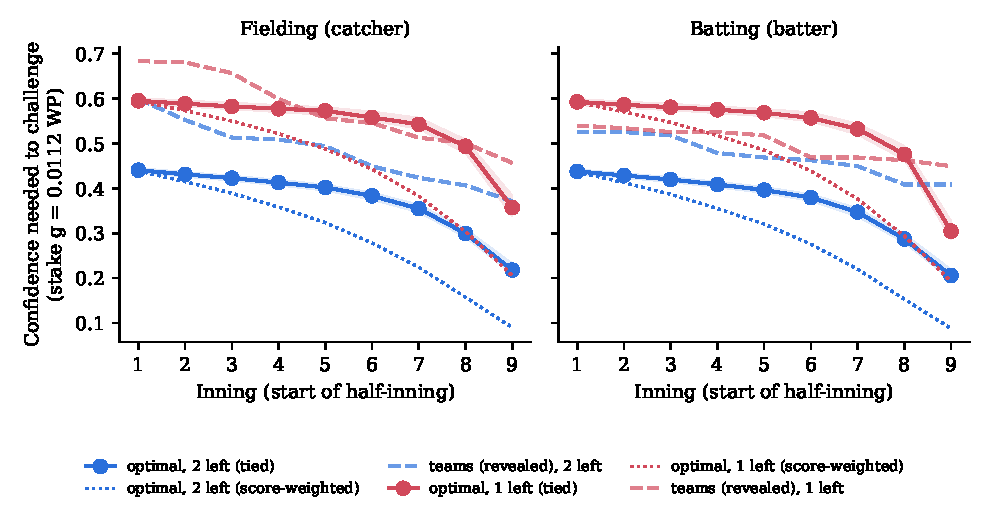
\includegraphics[width=.85\textwidth]{figures/fig_threshold}
\caption{Optimal confidence threshold for a challenge at the reference pitch, by inning and challenges held
(score-aware DP, main specification): tied score with 95\% bootstrap band, average over the score states visited in
2026, and teams' revealed thresholds. Panels are by challenging role; the values quoted in
Section~\ref{sec:bite} are at the start of the top of each inning and average the home and away DPs. In the first
inning the tied and score-averaged curves coincide by construction, since every game starts tied.}\label{fig:threshold}
\end{figure}

%% ============================================================================================================
\section{Evaluation of challenge policies}\label{sec:eval}

%% run-in heading set by hand: \paragraph adds a break penalty that strands the section title
\noindent{\itshape Estimand.}\hspace{1em}For a policy $\rho$ let $V(\rho)$ be the expected sum, over a team's 2026
season, of the stakes $g$ of the calls it flips, when the team follows $\rho$ on the real 2026 call stream, its
opponents' challenges are as recorded, and the player's information at a called pitch is the signal $s$, the count,
the inning, the score, the challenges held and the stake. The expectation is over the signal and the ruling given the
known truth, under the fitted model. Since $g$ is a jump in win probability, $V(\rho)$ is the policy's expected
contribution to wins under the accounting that sums the jumps along the recorded game; we check that accounting by
re-simulating games below. Wins lost are $V(\rho^\star)-V_{\rm obs}$, with $\rho^\star$ the DP benchmark and
$V_{\rm obs}$ the realised value of the teams' actual challenges, per team-season (the \NGamesABS{} games give 161.7
per team). Under a deterministic truth $V_{\rm obs}$ carries no outcome luck, only the luck of which pitches were
challenged. It is the gain to one team that adopts the policy while its opponents do not; wins are zero-sum, so these
gains do not add up to a league-wide gain. The benchmark depends on the behavioural model only through the decision
noise it reveals.

\paragraph{Design} Every policy is evaluated on the same simulated worlds. In each, every real 2026 called pitch
keeps its known truth $W$, the ruling is drawn with the mislabel rate $\pi$, the signal $s$ is drawn from the fitted
model, the belief $p$ is computed from $s$, and the policy decides along the real call stream at every challenge
opportunity (\NEvalOpp{} pitches), holding the challenges it would hold. Uncertainty comes from a game bootstrap
\citep{EfronTibshirani1993} with $B=\BootB$ that, in every replicate, refits the truth and perception model, re-solves
every DP and re-simulates. The intervals are percentile intervals of this resampling distribution: they include
parameter and sampling uncertainty, but not the model class (Section~\ref{sec:robust}). A joint bootstrap ($B=\JointBootB$)
that also re-estimates the WP engine, the stakes and the run laws of the DP from each resample gives \JointBootCI{}
(SD \JointBootSD, \JointBootRatio{} times the game bootstrap's), and a block bootstrap that resamples home-team months
instead of games, to allow for dependence through catchers, pitchers, umpire crews and the criterion's drift, gives
\BlockBootCI{} (SD ratio \BlockBootRatio). In \CovS{} seasons simulated from the fitted model, analysed with a smaller
bootstrap ($B=\CovB$, $R=\CovR$), the percentile interval covers that model's true gap to its own behavioural rule in
\CovRate\% \CovRateCI{} of them (Section~\Sref{sec:bootstrap}); its true gap, \CovGap{} wins, is close to the headline
because the model's teams earn about what the real ones did, and in it the mean bootstrap SD (\CovBootSD) exceeded the
SD of the point estimate across seasons (\CovPointSD), so the interval errs on the wide side. The value of an estimated optimal policy
is a maximum over policies, for which the bootstrap need not be valid in general \citep{LuedtkeVanDerLaan2016,LaberEtAl2014};
here the benchmark is unique and the value curve flat, and the coverage study is the check. Each replicate averages over
$R=\BootR$ simulated worlds and the point estimate over $R=\PointR$ (Monte Carlo standard error \LostMCSE{} wins). With
$B=\BootB$ the Monte Carlo error of the interval endpoints for the wins lost is about \CIEndSE{} wins, and the basic and
normal-approximation intervals agree with the percentile interval to within \CIAltMaxDiff{} at two decimals.
Section~\Sref{sec:policy} of the Supplementary Material \citep{JanousekPesta2026supp} gives the simulation, the
competitor rules and the bootstraps in detail.

\paragraph{Policies} The optimum is the score-aware DP. The one-line rule uses $\delta=\RuleDelta$. The best constant on
our grid at the point estimate is $\RuleDeltaBest$, with \ShareRuleBest\% of the optimum, and we keep $\delta=\RuleDelta$
throughout. (The constant was $0.01$ in an earlier
version of the analysis and moved to $0.008$ when the zone geometry was corrected; Table~\ref{tab:policies} keeps
the $0.01$ row.) Re-choosing $\delta$ in every bootstrap
replicate gives \ShareRuleResel\% \ShareRuleReselCI{} of the optimum; that propagates the variability of the choice
but, scored on the same games, not its optimism. For that we cross-fit: with every component (perception fit, belief
map, DP) estimated on March--June, the best constant there is $\FrozenDelta$, and frozen and applied to
July--September it gets \FrozenShare\% of that half's optimum and closes \FrozenGapClosed\% of the teams' gap. We
rebuild the public competitors on our model and data: the runs-objective rule of \citet{Namuduri2026runs} (challenge
when the run value of the flip exceeds the run cost of losing the challenge), the 48-cell threshold card of
\citet{Arora2026use} with its published thresholds and with each cell's median break-even from our DP (a reproduction
of its fitting procedure, not the value-maximising card), and the fixed 0.2-run rule published on Baseball Savant
\citep{Savant2026abs}, ``challenge iff $p\ge0.2/(0.2+\mathrm{RV})$'', with the run value RV of the flip from our own
run-expectancy engine rather than the league's RE288 table, and the same rule with its run cost tuned on a grid. All
rules use the same calibrated beliefs, which nobody using them in 2026 had, so this is a comparison of the rules'
targeting, not of their real-world use. We also simulate teams' fitted behavioural rule $s>\kappa(x)$.

\begin{table}[t]
\caption{Wins gained from challenges per team-season under each policy, 2026 MLB regular season, with 95\% game-bootstrap intervals
($B=\BootB$, model refit in every replicate). Wins lost: optimum minus the policy.}\label{tab:policies}
\centering\scriptsize
\resizebox{\textwidth}{!}{\begin{tabular}{p{3.9cm}cccc}
\toprule
 & \multicolumn{2}{c}{Primary} & \multicolumn{2}{c}{Comparator} \\
Policy & Wins & Challenges & Wins & Challenges \\
\midrule
Benchmark (primary intervention) & 3.85 [3.71, 4.06] & 2.71 & 3.98 [3.79, 4.11] & 2.70 \\
Teams' fitted rule $s>\kappa(x)$, simulated & 3.26 & 2.16 & 3.30 & 2.16 \\
\textbf{Observed 2026 (realised)} & 3.34 [3.17, 3.51] & 2.18 & 3.34 [3.17, 3.51] & 2.18 \\
\midrule
\textbf{Accounting index} & 0.51 [0.38, 0.63] & & 0.63 [0.51, 0.76] & \\
\bottomrule
\end{tabular}
}
\end{table}

\begin{figure}[t]
\centering
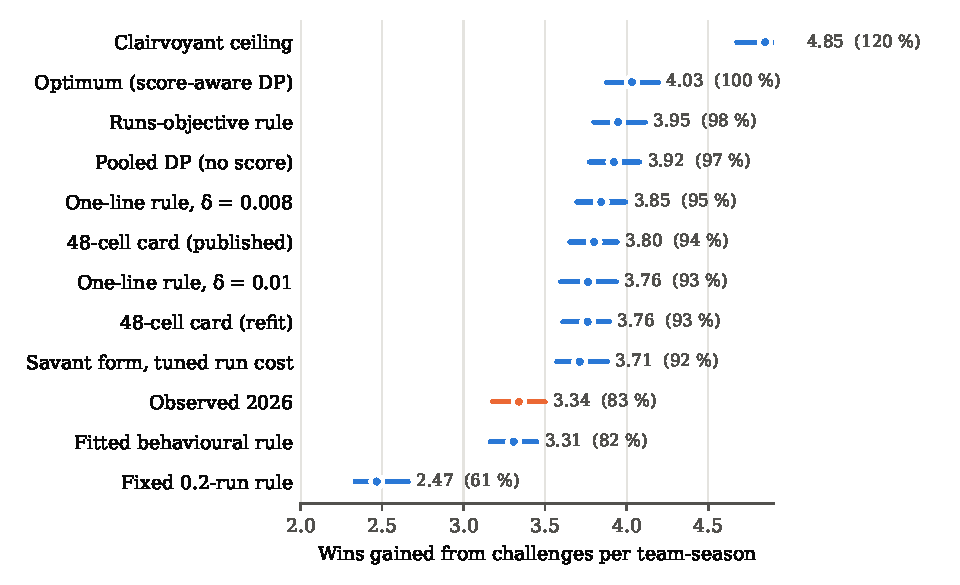
\includegraphics[width=.9\textwidth]{figures/fig_policies}
\caption{Wins gained from challenges per team-season (dots) with 95\% game-bootstrap intervals; share of the optimum
in parentheses. Orange: observed 2026 behaviour.}\label{fig:policies}
\end{figure}

\paragraph{Results} Table~\ref{tab:policies} and Figure~\ref{fig:policies} give the results. The optimum gains
\WOpt{} \WOptCI{} wins per team-season from challenges, at \NOpt{} challenges per team-game. Teams realised \WObs{}
\WObsCI{} at \NObs, so they left \WinsLost{} \WinsLostCI{} wins per team-season against the benchmark. Batters account
for \WinsLostBatter{} \WinsLostBatterCI{} and catchers and pitchers for \WinsLostFielder{} \WinsLostFielderCI. The
optimum challenges \NMorePct\% more often than teams, but that is not where most of the loss comes from: the one-line
rule makes \NRule{} challenges per team-game against the teams' \NObs{} and still recovers \RuleGapClosedPct\% of the
gap, while the optimum's extra challenges add the remaining \OptMinusRule{} wins. Because the policies differ in timing,
success and the challenges they hold as well as in frequency, this is a comparison at nearly equal frequency, not a
unique decomposition of the gap; together with the threshold slopes of Section~\ref{sec:bite} it says that the loss
lies mainly in targeting. The fitted behavioural rule simulated in the model earns \WFitRule{} \WFitRuleCI{} wins
against the \WObs{} realised, so the model's teams are about as skilled as the real ones, and measured against the
simulated rule the loss is \LostFitRule{} \LostFitRuleCI. With a criterion linear in $\log g$ the simulated rule
earned less than teams realised; the misfit sat in the top fifth of stakes (Section~\Sref{sec:behaviourgap}), and the
piecewise criterion of the main model removes it while leaving $\sigma_r$ practically unchanged. A loss of this size is
small against the luck in a season's standings: \citet{LopezEtAl2018} find MLB game outcomes among the most random in
North American sport. Unlike that luck, however, it is a systematic loss from decisions the teams control, and the
clairvoyant ceiling (\WClair) shows that no richer state could raise the benchmark by more than \ClairGap.

The value curve is flat. The one-line rule, with one constant and no state, gets \ShareRule\% with $\delta$ fixed at
\RuleDelta; the runs-objective rule gets \ShareRuns\% \ShareRunsCI{}, and is the strongest simple competitor; the
48-cell card gets \ShareCardRefit--\ShareCardPub\%, because its cells cut the stake into terciles and so lose the
leverage scaling that the cutoff~\eqref{eq:cutoff} requires. Flat in the state does not mean flat in the constant: with
$\delta=0.01$ instead of \RuleDelta{} the rule gets \ShareRuleOld\%. The fixed 0.2-run rule, which Baseball Savant
publishes as the break-even for a challenge, gets only \ShareSavant\% \ShareSavantCI, below the \ShareObs\%
\ShareObsCI{} teams achieved, and challenges far too rarely (\NSavant{} per team-game). Most of that is the constant:
with the run cost tuned to \SavantTunedC{} runs the same form gets \ShareSavantTuned\% \ShareSavantTunedCI; the rest
is that a fixed run cost charges the same price in the first inning as in a tied ninth and prices the stake in runs,
not wins.

\paragraph{Causal accounting} \citet{Arora2026use} objects that summing stakes along the recorded game is not causal:
after a flipped call the rest of the game would have been different. The path sum equals the expected effect of the
flips on winning only if the WP engine is the conditional win probability given the game state \emph{and} the states
are visited as the policy would visit them, which the recorded game does not guarantee once policy and play part.
We therefore re-simulate. For every policy, simulated world and team-game we find the first pitch at which the policy's
game and the recorded game part: the first call that exactly one of them flips, either a call the policy overturns and
the team left standing or one the team overturned and the policy would have left (\CausalSkipShare\% of the branch
points for the optimum). Up to that pitch the two games coincide. From it we continue the game in a pitch-level
simulator twice, once with each call, with the team following the policy with the challenges it holds and the opponent
following its fitted behavioural rule, and difference the two by common random numbers; the difference includes
everything the flip changes downstream: the later counts, both teams' later opportunities and gains, and the
challenges the team still holds. The simulator has pitch events and in-play outcomes by count, outs and bases, plus
baserunning between pitches, all estimated from 2026 Statcast. We average over $K=\CausalK$ play-outs per world and
$R=\CausalR$ draws of the signals. The simulator reproduces the engine's win probabilities in every decile, and a flip
moves its win probability by \SimGShareRun\% of $g$. Valued this way, the optimum's value differs from the path sum by
$\CausalMinusPath$ \CausalMinusPathCI{} wins per team-season, every policy is within $\pm\CausalMaxAbs$, and teams lose
\CausalLost{} \CausalLostCI. The check is internal to the model: it cannot detect what the engine and the simulator
share (no team, park or matchup effects, no strategic response to a flip), which Section~\ref{sec:discussion} lists
as limitations, and it continues the game after the branch with the fitted rule for the opponent.

Counting simulated wins in the two worlds instead of differencing the values of later challenges gives \BinaryLost{}
\BinaryLostCI, also within a few hundredths of the path sum; the difference between the two estimators,
$\BinaryMinusRB$ \BinaryMinusRBCI, is what the remaining \SimGShareRunGap\% mismatch between simulator and engine in
$g$ predicts (Section~\Sref{sec:causalgap}).

%% ============================================================================================================
\section{Robustness of the perception model}\label{sec:robust}

Perception noise is the parameter the conclusions are most sensitive to, because the value of a challenge falls
quickly as perception gets worse. The question is how wrong $\sigma_r$ would have to be to overturn the conclusion. The wins
lost fall to $0.25$ only if $\sigma_r$ is \BreakEvenPct\% larger than estimated for both sides. The profile likelihood
rejects that by \BreakEvenLLBatter{} log-likelihood points for batters and \BreakEvenLLCatcher{} for catchers; even
a $10\%$ error costs \ProfileTenBatter{} and \ProfileTenCatcher{} points. (The profile is computed on the baseline
model of Table~\ref{tab:variants}, within which it rules out only that model's own misspecification of the scale; the curve of wins lost against $\sigma_r$ is in Section~\Sref{sec:breakeven} of the Supplementary Material \citep{JanousekPesta2026supp}.) We
check the model in five more ways.

\emph{Alternative noise laws.} Logistic and $t_{10}$, $t_5$, $t_3$ errors are worse than the Gaussian by
\DLLRejLo--\DLLRejHi{} log-likelihood points at the same parameter count in the baseline model
(Table~\ref{tab:variants}) and by \DLLRejMainLo--\DLLRejMainHi{} in the main model (Section~\Sref{sec:perception}). Region-specific
$\sigma_r$ and $\kappa$ are supported; a $\sigma_r$ that grows with distance from the edge adds almost nothing. Every
homogeneous probit model that fits at least as well as the Gaussian baseline gives \SpreadLo--\SpreadHi{} wins lost; the
rejected heavy-tailed models,
simulated with signals drawn from their own noise laws, give \SpreadRejLo--\SpreadRejHi. A nonparametric check does not depend on any family: by side and zone region, the
isotonic regression of the challenge indicator on $w$ stays within \IsoMaxGap{} percentage points of the fitted
probit curve, and the probit curve lies inside the pointwise 95\% bootstrap band of the isotonic fit at
\IsoBandLo--\IsoBandHi\% of the grid points (Figure~\Sref{fig:isotonic}); these are pointwise graphical checks, not a
simultaneous test. The curve levels off below one for pitches far from the zone, which a lapse rate $\lambda$, with
$\Prob(\text{challenge}\mid w)=(1-\lambda)\Phi\{(w-\kappa)/\sigma_r\}$ \citep{WichmannHill2001}, captures (before the
join check of Section~\ref{sec:data} the plateau was largely mis-joined pitches; Section~\Sref{sec:perception}). It
improves the BIC of the linear-criterion model by \LinLapseDBIC{} and of the main model by \LapseDBIC{}
(\LapseDLL{} log-likelihood points for \LapseK{} parameters), with $\lambda$ at \LapseBatter\% for batters and
\LapseCatcher\% for catchers and $\sigma_r$ \LapseSrDropPct\% and \LapseSrDropPctCatcher\% lower (\LapseSrBatter{}
and \LapseSrCatcher\,in). A criterion with an extra rise below $g=0.001$ and a $\sigma_r$ varying with $\log g$ both make the main
model's BIC worse (by \GlowDBICAbs{} and \SrGDBICAbs). A lapse is a challenge not made on a call the
player sees as wrong, and what the benchmark should assume about it is a choice of intervention. If the player's
lapses could be removed, the wins lost under the lapse model are \LapseLost; if they stay and only the decision rule
changes, they are \LapseLostKept. Its own behavioural rule, simulated with the lapses, earns \LapseFitRule{} against
\WObs{} realised.

\emph{Player heterogeneity.} Player random effects on $(\kappa,\log\sigma_r)$ improve the likelihood by \DLLREvsMain{}
points over the main model and have the best BIC (\BICRE; a lapse rate on top improves it by \RELapseDBIC). They sit
mostly in the criterion (SD \REKappaSDBatter\,in for batters, \REKappaSDCatcher\,in for catchers) rather than in the
decision noise (SD of $\log\sigma_r$ \RELogSrSDBatter{} and \RELogSrSDCatcher). With each player's belief calibrated to
their own noise level (approximately: within five noise quintiles), the wins lost are \PPLost{} \PPLostCI{} (bootstrap
with empirical-Bayes redraws of the player effects, drawn independently for $\kappa$ and $\log\sigma_r$, without refits,
$B=\PPB$; the same bootstrap gives \MainNorefCI{} for the main model, against \WinsLostCI{} with refits). The one-line
rule still gets \PPRuleShare\% of that optimum.

\emph{Model class.} Across the models whose BIC is at least as good as the main model's (the main model, the lapse
model and the player-effects models), the wins lost range over \SpreadAllLo--\SpreadAllHi. This spread, not the
sampling interval of any one model, is the larger part of the uncertainty about the size of the loss; the qualitative
conclusions (a flat value curve, a one-line rule near the benchmark, leverage-blind thresholds, the 0.2-run rule below
unaided play) hold in every one of them.

\emph{Out of sample.} Table~\ref{tab:oos} (details in Section~\Sref{sec:oos}) fits the main model to March--June and
predicts July--September. The decision noise transfers, and so does the overturn rate of the pitches the model would
challenge. Catchers challenged $\OOSCatcherExcess\%$ more in the second half than the first-half fit predicts: their
criterion shifted during the season, whether by learning, coaching or roster changes. Against its own half the
first-half benchmark puts the second-half loss at \OOSTestLost{} wins per team-season (\OOSTestLostOwn{} with
second-half parameters).

\begin{table}[t]
\caption{Out-of-sample and external-league checks of the perception model (main specification). Triple-A and
spring-training feeds report the ABS system's own coordinates. Overturn rate: among the pitches the model would have
challenged, against the observed rate among the challenges made. MLB 2026 values: $\sigma_r=\SrBatter$ and
\SrCatcher\,in.}\label{tab:oos}
\centering\small
\begin{tabular}{lrrcc}
\toprule
Fit sample $\to$ evaluation & \multicolumn{2}{c}{$\sigma_r$ (in)} & \multicolumn{2}{c}{Overturn rate, model / obs. (\%)} \\
 & batter & catcher & batter & catcher \\
\midrule
MLB 2026 Mar--Jun $\to$ Jul--Sep & 2.88 & 1.92 & 50.4 / 50.2 & 58.3 / 57.7 \\
Triple-A 2025 (refit) & 3.22 & 2.09 & 46.3 / 45.0 & 54.6 / 53.8 \\
Spring training 2026 (refit) & 3.78 & 2.18 & 46.3 / 45.7 & 57.5 / 59.5 \\
\bottomrule
\end{tabular}

\end{table}

\emph{Other leagues and coordinates.} In Triple-A 2025 and spring training 2026 the feeds carry the ABS system's own
measurements, which also reproduce the rulings almost exactly. Separate fits of the main model give decision noise of
\AAASrBatter{} and \AAASrCatcher\,in in Triple-A and \SpringSrBatter{} and \SpringSrCatcher\,in in spring training,
\AAASrPctLo--\AAASrPctHi\% and \SpringSrPctLo--\SpringSrPctHi\% above MLB; leagues, seasons and measurement systems
differ, so we read these as external fits, not as a transport test. Rebuilding 2026 on the MLB feed's own
coordinates, projected to the plate midpoint, reproduces \GeomReproFeed\% of the rulings and gives \FeedSrBatter{}
and \FeedSrCatcher\,in, against \SrBatter{} and \SrCatcher\,in on Statcast.

\emph{Miscalibrated beliefs.} Overconfidence cannot be tested from challenge choices (Section~\ref{sec:model}) and does
not change the estimand, which is the best policy given the same signal. Under a flat-prior belief map the implied
threshold slopes on $\log g$ are \SlopeFlatBatter{} and \SlopeFlatCatcher: whatever players believe, their
thresholds barely respond to leverage.

\subsection{The 2026 postseason}\label{sec:post}
The postseason is an out-of-sample test with higher stakes: every parameter, the belief map and the DP are held at
their regular-season values. We use the \PostGames{} postseason games completed by 17 October 2026
(\PostWCGames{} Wild Card, \PostDSGames{} Division Series and \PostLCSGames{} League Championship Series games; the World
Series had not started), with
\PostCalled{} called pitches and \PostCh{} challenges, \PostPerTeamGame{} per team-game against \RSPerTeamGame{} in the
regular season. The published zone rule reproduces every postseason ruling on Statcast's coordinates. The
postseason has no runner on second in extra innings, so its stakes come from the WP engine solved without it; the
policy is the regular-season one, frozen, so this is a transport test of that policy rather than a postseason optimum.
Table~\ref{tab:post} gives the results.

\emph{Perception is not contradicted.} With regular-season parameters held fixed, the model predicts \PostChPredBatter{} batter
challenges against \PostChObsBatter{} observed, and its challenge log-score skill over a constant challenge
probability is \PostSkillBatter{} for batters and \PostSkillCatcher{} for catchers, at least as high as in the regular
season (\PostSkillRSBatter{} and \PostSkillRSCatcher). Catchers challenged more often than predicted ($z=\PostChZCatcher$), but a fit to games after the All-Star break (14 July) alone predicts their count to within $z=\PostChZHalfCatcher$: the excess continues the in-season shift above. Refitting
$\sigma_r$ on the postseason alone gives \PostSrBatter{} \PostSrBatterCI\,in for batters and \PostSrCatcher{}
\PostSrCatcherCI\,in for catchers, against regular-season values of \PostSrRSBatter{} and \PostSrRSCatcher\,in; these
refits hold the other parameters at their regular-season values, so their intervals are conditional, and the $z$
statistics treat pitches as independent.

\emph{Thresholds still ignore the stakes.} Refitting the criterion's intercept and its coefficient on $\log g$ to the
postseason challenges gives an implied threshold slope on $\log g$ of \PostSlopeBatter{} \PostSlopeBatterCI{} for
batters and \PostSlopeCatcher{} \PostSlopeCatcherCI{} for catchers, the same as in the regular season and far
below the optimum's \OptSlopeBatter{} and \OptSlopeCatcher. Higher stakes did not make players more selective about leverage.

\emph{Value.} Because
challenges do not carry over between games, maximising the probability of winning a series is, within a game, the
same as maximising the game's win probability, so the regular-season optimum is still the right benchmark
(Section~\Sref{sec:postseason}). Descriptively, teams lost \PostLostWP{} \PostLostWPCI{} win probability per team-game
against that optimum, against \RSLostWP{} in the regular season; with \PostGames{} games the interval is wide and
contains both zero and the regular-season value, so it does not discriminate between them.

\begin{table}[t]
\caption{The 2026 postseason through 17 October, with the regular-season model held fixed unless
stated. Log-score skill: improvement of the challenge log score over a constant challenge probability. Intervals are
95\% intervals from the asymptotic normal law of the refitted parameters; the optimum's thresholds have slope
\OptSlopeBatter{} (batters) and \OptSlopeCatcher{} (catchers) on $\log g$ in the same regression.}\label{tab:post}
\centering\small
\resizebox{\textwidth}{!}{\begin{tabular}{lcc}
\toprule
 & Batters & Catchers and pitchers \\
\midrule
Challenges, observed / predicted ($z$) & 60 / 61.5 ($-0.2$) & 96 / 79.6 ($+2.2$) \\
\quad predicted from a post-All-Star-break fit ($z$) & 62.4 ($-0.3$) & 88.4 ($+1.0$) \\
Challenge log-score skill, postseason / regular season & 0.38 / 0.30 & 0.46 / 0.42 \\
$\sigma_r$ (in), postseason refit / regular season & 2.69 [2.43, 2.97] / 2.88 & 1.93 [1.75, 2.13] / 1.82 \\
Threshold slope on $\log g$, postseason refit / regular season & 0.06 [\ensuremath{-}0.06, 0.18] / 0.08 & 0.04 [\ensuremath{-}0.08, 0.17] / 0.04 \\
\bottomrule
\end{tabular}
}
\end{table}

%% ============================================================================================================
\section{Discussion}\label{sec:discussion}

\paragraph{What a team should do} Challenge when $p\ge\RuleDelta/(g+\RuleDelta)$ with $g$ in win probability. The
rule needs the stake in WP, which every team's analysts already compute, and an honest confidence. The second is the
hard part: the benchmark gives every player a calibrated belief, which nobody has been shown to hold, and a
practical version is a criterion on the signal that falls with the stake, for a batter from about \KappaLowBatter\,in
in the lowest stake quintile to \SRuleHighBatter\,in in the highest, against the teams' \KappaHighBatter\,in
(Table~\Sref{tab:mechanism}). The rule recovers most of what the DP offers because mis-pricing the continuation value
is a second-order error (Theorem~\ref{thm:flat}), and a constant chosen on half a season keeps its share on the other
half. A rule with a state-dependent run cost of a challenge \citep{Namuduri2026runs} does better (\ShareRuns\%) but
needs a DP to price the challenge. A fixed run cost of 0.2 runs, the break-even published on Baseball Savant, is the
one choice we can rule out.

\paragraph{Limitations} (i) The WP engine is league-average, has no home-field term (adding one changes the wins lost
by $\HomeFieldLostChange$) and is estimated from the same season; its count transitions are empirical
continuations, not interventions on the count, and its level calibration does not validate the differences between a
ball and a strike in sparse high-leverage states. The joint bootstrap covers its sampling uncertainty, not its
structure. (ii) The counterfactual keeps the real call stream and the opponents' play fixed, apart from the
re-simulation of Section~\ref{sec:eval}, whose simulator shares the engine's structure, so that check verifies the
accounting, not the engine. (iii) The DP state is the half-inning, the score at its start, the opportunity and the
challenges held; outs, bases and count enter only through the stake. The clairvoyant ceiling bounds what a richer
state could add, but not tightly. (iv) The perception model treats the challenger as a single decision-maker with a
known noise level and a calibrated belief; $\sigma_r$ is decision noise, not eyesight, and whether a lapse could be
trained away is a choice of intervention (Section~\ref{sec:robust}). (v) The known truth depends on the 2026 Statcast
convention; the feed's own coordinates give the same decision noise. (vi) Teams' criteria shifted during the season,
so the 2026 gap may shrink in 2027, which is a testable prediction. (vii) The postseason check rests on \PostGames{}
games. (viii) The optimum maximises the probability of winning the game. A player who weighs their own plate
appearance, or a manager who keeps a challenge in reserve for its own sake, has a different objective, and part of the
leverage-blindness may reflect it; we do not estimate such preferences, as \citet{SandholtzEtAl2024} do for fourth
downs. (ix) The coverage study has 50 seasons, so it cannot distinguish 90\% from 99\% coverage.

\paragraph{Cricket} Cricket's Decision Review System keeps a review that ends in ``umpire's call'', the same retention
structure. An exploratory application to Cricsheet ball-by-ball data \citep{Cricsheet}, in
Section~\Sref{sec:drs} of the Supplementary Material, lacks the paper's central device: the ball-tracking truth is not
public, so the truth enters as a latent margin and the decision noise is weakly identified. With that caveat the value
curve is again flat and the optimal threshold again moves with the state; the losses are small and their intervals
include zero. For the economics of DRS decisions see \citet{Shivakumar2018}.

\paragraph{Prior work} The optimal retention DP, the size of the gap between observed and optimal play and
role-specific perception noise are in public, non-peer-reviewed work that predates this paper
\citep{Arora2026use,Namuduri2026runs,Kirby2026economy,Hires2026sdt,Tango2026naive}; descriptive analyses of the first
season include \citet{LeeEtAl2026abs}, \citet{Baumann2026money} and \citet{Oler2026count}. Our estimates of the gap and
of the noise agree with theirs in order of magnitude. The umpire's zone itself has a statistical literature:
\citet{ZimmermanEtAl2019} model its shape, \citet{DeshpandeWyner2017} the catcher's framing of it, and
\citet{ParsonsEtAl2011}, \citet{KimKing2014} and \citet{ChenEtAl2016} the biases of the umpires who call it; the
challenger's criterion is the mirror image of those models. The estimand is a sum of win-probability increments, as in
openWAR and nflWAR \citep{BaumerEtAl2015,YurkoEtAl2019}, and the comparison of observed with optimal sports decisions
goes back to \citet{Romer2006}. Inference for the value of an estimated optimal policy is the dynamic-treatment-regime
problem \citep{Murphy2003,LaberEtAl2014,LuedtkeVanDerLaan2016} and, for a fixed rule class, empirical welfare
maximisation \citep{KitagawaTetenov2018}. What we add is a known truth for every called pitch, which turns the
selected challenge data into a binary-response problem; the evidence that most of the gap lies in which pitches are
challenged; the theory of retained challenges; and the evaluation of every public rule on one model with refit and
joint uncertainty, a clairvoyant ceiling and a re-simulation from the first divergence.

%% ============================================================================================================
\section{Reproducibility}\label{sec:repro}

The code and the outputs are supplied as a supplement to this paper and are also available at \url{https://github.com/HeirOfIsildur/abs-challenge-policy}. The raw MLB Stats API and
Statcast data and the Cricsheet data are public and are not redistributed; the scripts \texttt{src/fetch\_*.py}
re-fetch them, and the README lists the run order; \texttt{results/manifest.json} records the commit, the pinned
package versions (\texttt{requirements-lock.txt}) and checksums of the raw inputs used, since public feeds can be
revised. Every number in this paper is written by
\texttt{paper/make\_numbers.py} from the outputs in \texttt{results/}, and \texttt{make -C paper} rebuilds the tables,
figures and PDF. The exact algebra (the cutoff, the identification of the deterministic-truth model and its
tracking-noise bound, Theorems~\ref{thm:mono}--\ref{thm:flat} and the causal decomposition) is checked in
Mathematica~\ProofsVersion{} by the scripts in \texttt{wolfram/}; these verify the algebra, not the assumptions under
which a result applies to the data. Section~\Sref{sec:kernel} of the Supplementary Material \citep{JanousekPesta2026supp}
lists the checks and their outcomes.

\begin{acks}[Acknowledgments]
Pitch-tracking data are from MLB's Statcast via Baseball Savant and challenge events from the MLB Stats API; cricket
data are from Cricsheet.
\end{acks}

\begin{funding}
The research of Jan Janou\v{s}ek and Michal Pe\v{s}ta was supported by the Czech Science Foundation (GA~\v{C}R)
No.~27-25747L and the Charles University Grant Agency (GA~UK) No.~188325. The funders had no role in the study design,
the collection, analysis and interpretation of the data, the writing of the manuscript or the decision to submit it.
\end{funding}

\begin{acks}[Declaration of generative AI and AI-assisted technologies in the writing process]
During the preparation of this work the authors used large language models (Anthropic's Claude and OpenAI's GPT
models) to improve the English of the manuscript, as non-native speakers; to check derivations, formulas and
arithmetic; and to assist in writing and reviewing the analysis code. After using these tools, the authors reviewed and
edited the content as needed and take full responsibility for the content of the publication.
\end{acks}

\begin{supplement}
\stitle{Proofs, symbolic verification and additional results}
\sdescription{S1: full proofs of Theorems~\ref{thm:mono}--\ref{thm:flat} and of a theorem comparing retained with
consumable challenges, with the status of every theoretical statement. S2: the Mathematica scripts and a table of every
symbolic check and its outcome. S3: the geometry and data audit (coordinate convention, reproduction of the ABS rulings by
edge, side and month, the mismatches, the challenges left against the feeds' counters, the extra-inning rule). S4: the
perception model in full (all variants, player random effects, out-of-sample halves, Triple-A and spring training,
known-truth recovery, wins lost against perception noise). S5: policy evaluation (causal re-simulation, the win-count estimator and
the simulator--engine decomposition, competitor rules, the flat-optimum bound on the calibrated pools, bootstrap and Monte Carlo
error). S6: the 2026 postseason in full. S7: the exploratory cricket DRS application.}
\end{supplement}
\begin{supplement}
\stitle{Code and results}
\sdescription{A zip archive of the code repository at the version used for this paper: the data-fetching scripts, the
pipeline, the Mathematica scripts in \texttt{wolfram/}, the outputs in \texttt{results/} from which every number, table and
figure is generated, and the manuscript sources. The same code is public at
\url{https://github.com/HeirOfIsildur/abs-challenge-policy}. The raw MLB and Cricsheet data are not included; the fetch
scripts re-download them from the public sources.}
\end{supplement}

\bibliographystyle{spr-ims-nameyear}
\bibliography{refs}

\end{document}
